\chapter{Implementación a nivel de microarquitectura}

En el capítulo \ref{sec:cap_arqs} se analizaron diferentes tipos de arquitecturas existentes para el
cómputo de la DFT y se seleccionaron dos arquitecturas para ser implementadas. A su vez fueron analizadas
algunas alternativas para la implementación de diferentes aspectos del cómputo.

En este capítulo se describe la implementación a nivel de microarquitectura de los
módulos que componen las dos arquitecturas seleccionadas y la forma en que esos módulos se
interconectan. También se presentan las herramientas utilizadas para el diseño e implementación
de las arquitecturas.

El proceso de desarrollo se dividió en tres etapas. Primero, una vez seleccionadas las
arquitecturas, se conformó un diagrama en bloques identificando los módulos constitutivos, luego se implementó cada
uno de esos módulos realizando pruebas de funcionamiento en cada uno en forma individual y se
finalizó con la integración gradual de todos los módulos realizando las pruebas pertinenetes para
verificar cada etapa de integración. Una vez integrada completamente cada arquitectura se realizaron
tests de verificación y validación, cuyos resultados se presentan en el capítulo \ref{sec:simsec}.

Al implementarse dos arquitecturas separadas se analizará en primera instancia las particularidades
de cada arquitectura, como su unidad de control, memoria y sumadores, y luego se
analizarán los módulos compartidos por ambas arquitecturas.

\section{Arquitectura Radix-2}

\subsection{Descripción general}

Como se explicó en la sección \ref{sec:radix} al implementar un algoritmo radix-2 de $N$ puntos en
forma iterativa se utiliza el mismo módulo \textit{butterfly} para cada una de las etapas del cómputo de
la radix, debiendo esperar $log_2(N)$ ciclos de \textit{clock} entre cada punto de entrada y entre
cada punto de salida, durante los cuales se realiza una operación de cada etapa.

La figura \ref{fig:r2_8_c3} muestra el esquema presentado en la sección \ref{sec:radix}. Allí se
identifican las diferentes etapas del cómputo, en cada ciclo de \textit{clock} se ejecuta
sucesivamente una operación de cada etapa, por lo que luego de $log_2(N)$ ciclos se habrá ejecutado
una operación de cada etapa y se vuelve a la primera.

\begin{figure}[htb!]
        \centering
        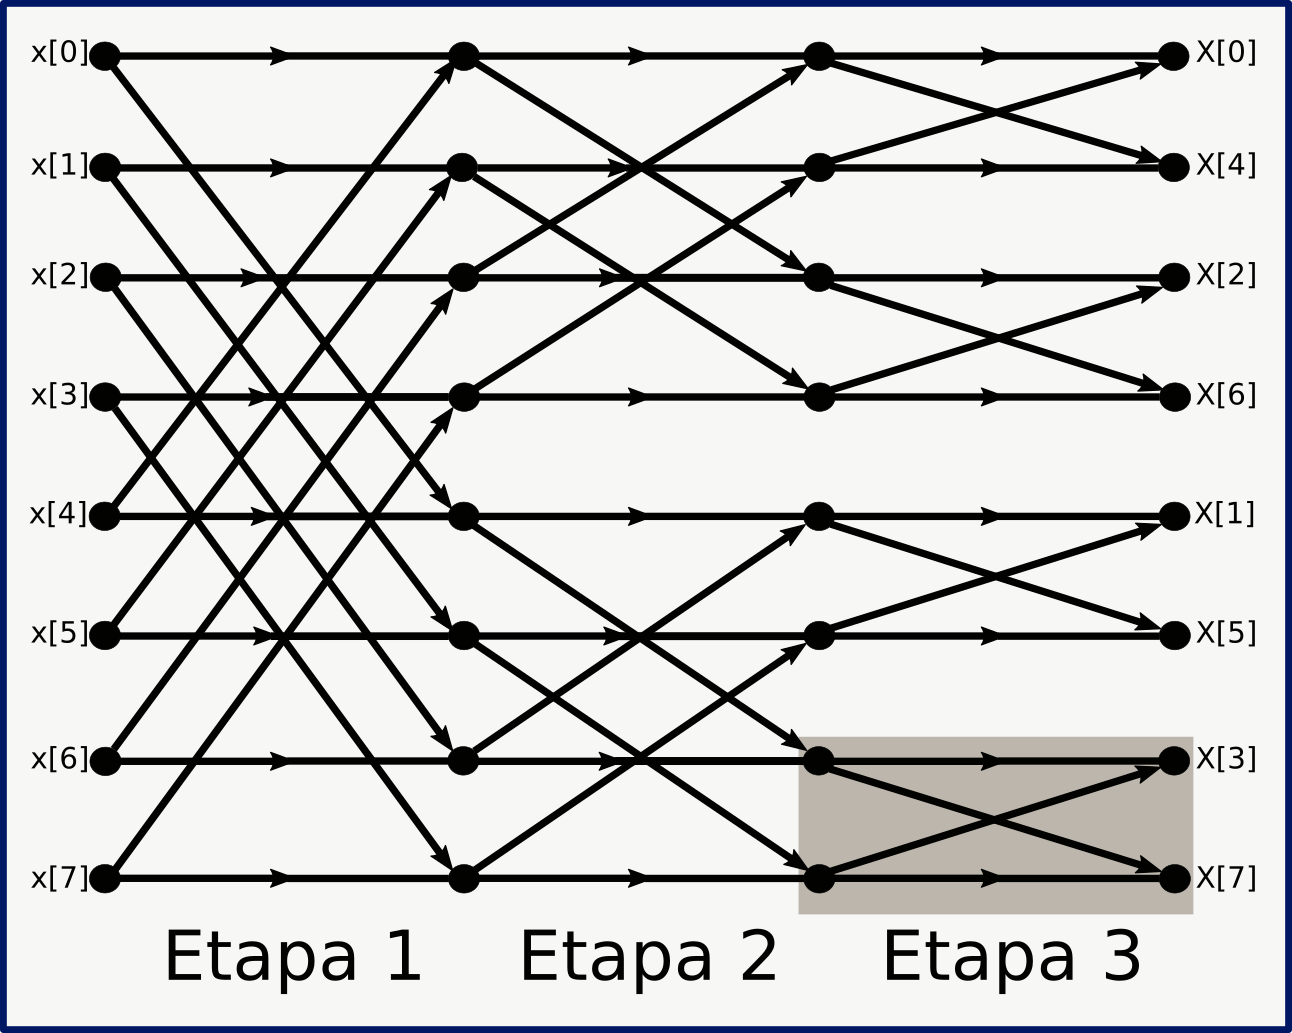
\includegraphics[width=10cm]{./figures/r2_8_diag.png}
        \caption{FFT Radix-2 de 8 puntos}
        \label{fig:r2_8_c3}
\end{figure}

Dado que los datos ingresan de a uno en la arquitectura, deben almacenarse en memoria hasta que se
tiene el dato necesario para realizar una operación aritmética. Es importante notar que en cada
etapa de cálculo aritmético se utilizan dos datos como entradas al \textit{butterfly} y se obtienen
dos datos como resultados, de los cuales uno se utiliza en la etapa siguiente y el otro se almacena en memoria.

En la arquitectura iterativa a implementar, se ejecuta en cada ciclo de \textit{clock} una operación
de una etapa, pasando a la siguiente etapa en el ciclo de \textit{clock} siguiente, de forma que al
transcurrir $\log_2(N)$ ciclos de \textit{clock} se ejecutó una operación de cada etapa volviendo a
la etapa inicial.

La figura \ref{fig:radix2blocks} muestra un diagrama en bloques de la arquitectura radix-2
iterativa. Se diferencian claramente tres partes: la memoria, la unidad aritmética, compuesta por el
\textit{butterfly} y el multiplicador, y la unidad de control. Los distintos colores de los bloques
indican si el mismo es un circuito combinacional, un circuito secuencial o una unidad de
almacenamiento. Este diagrama es a modo de esquema general y es del que se partió para el
desarrollo de la arquitectura, al final de esta sección se presenta el diagrama del
\textit{datapath} detallado con las señales de control necesarias para su funcionamiento.	


\begin{figure}[htb!]
        \centering
        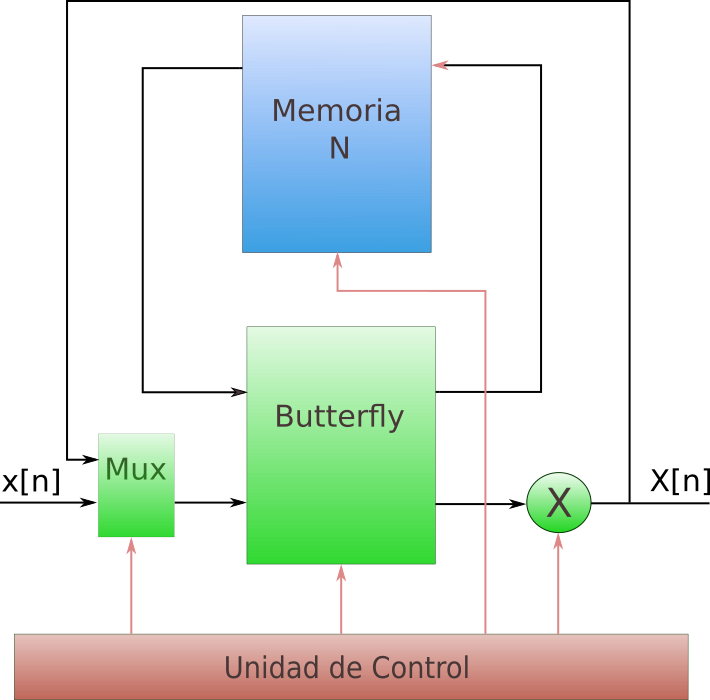
\includegraphics[width=10cm]{./figures/radix2blocks.png}
        \caption{Diagrama simplificado de la arquitectura radix-2 iterativa}
        \label{fig:radix2blocks}
\end{figure}

\subsection{Memoria} \label{sec:r2mem}

Debido al tipo de acceso a los datos se decide implementar una memoria de almacenamiento de tipo
RAM de doble acceso (\textit{dual port RAM}) permitiendo realizar simultáneamente operaciones de lectura y escritura. Las interfaces son las típicas para
esta memoria y se describen en la figura \ref{fig:dualPortRam}.

\begin{figure}[htb!]
        \centering
        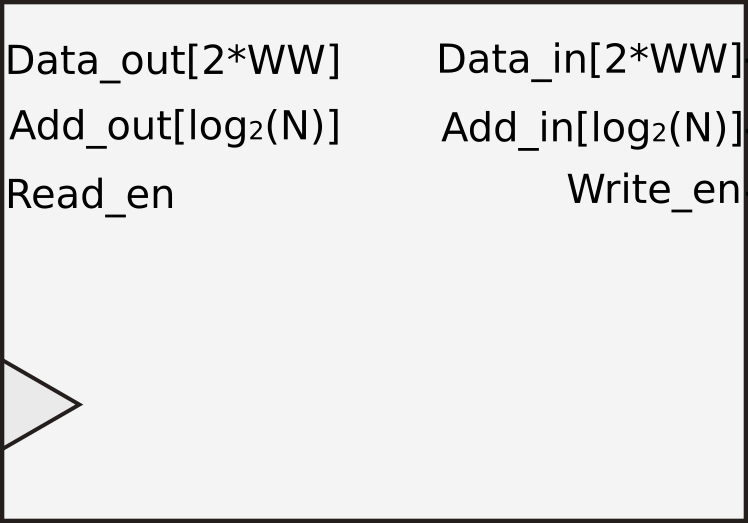
\includegraphics[width=5cm]{./figures/dportRam.png}
        \caption{Dual Port RAM}
        \label{fig:dualPortRam}
\end{figure}

En la figura \ref{fig:dualPortRam} se muestran los buses de entrada y salida indicando su tamaño
entre corchetes.
El parámetro \textit{WW} corresponde al parámetro global \textit{WORD\_WIDTH} e indica el ancho de palabra de la
arquitectura. El parámetro \textit{N} indica la cantidad de puntos para la que se configura la
arquitectura. Las variables a almecenar son complejas, por lo que se concatenan la parte real y la
imaginaria y se guardan en memoria como un único valor. De este modo el tamaño de palabra de la 
memoria es el doble del tamaño de palabra de la arquitectura, teniendo también sus buses de entrada 
y salida el doble de ancho que los demás buses de la arquitectura.

\subsection{Butterfly}

Para la arquitectura radix-2, el \textit{butterfly} debe computar con dos operandos según la
siguiente ecuación:

\begin{equation}
\begin{split}
c &= a+b \\
d &= a-b
\end{split}
\label{eq:butterf}
\end{equation}

Siendo todas las variables complejas. En la figura \ref{fig:butterfly_esq} se muestra el esquema del
bloque \textit{butterfly}, compuesto por un sumador y un restador complejos.

\begin{figure}[htb!]
        \centering
        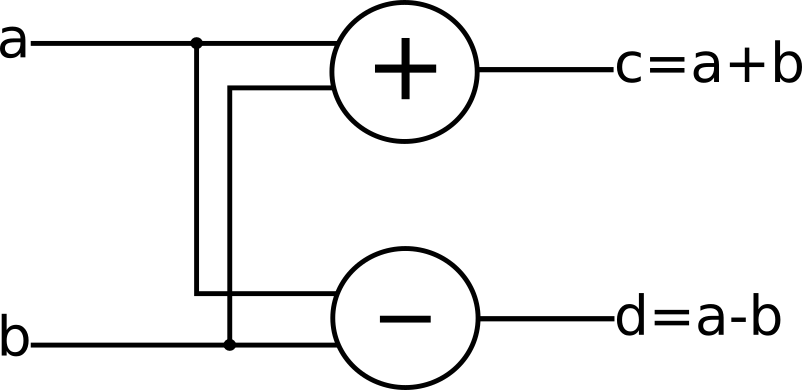
\includegraphics[width=6cm]{./figures/butterfly_esq.png}
        \caption{Esquema del bloque butterfly}
        \label{fig:butterfly_esq}
\end{figure}

\subsection{Datapath} \label{sec:datapath}

En la figura \ref{fig:datapath} se muestra el \textit{datapath} de la arquitectura radix-2. Se muestra el
butterfly como un sumador y un restador, y un multiplicador genérico que puede ser implementado como
un procesador cordic o como un multiplicador complejo. Dado que en las etapas intermedias y en la
etapa final se debe operar con un dato de la etapa anterior se coloca un registro (\textit{delay
register}) donde se almacena ese dato durante un ciclo de clock para ser utilizado en la etapa siguiente. 
A la salida se le coloca un registro similar para facilitar la
sincronización con otros elementos del entorno de la arquitectura.

\begin{figure}[htb!]
        \centering
        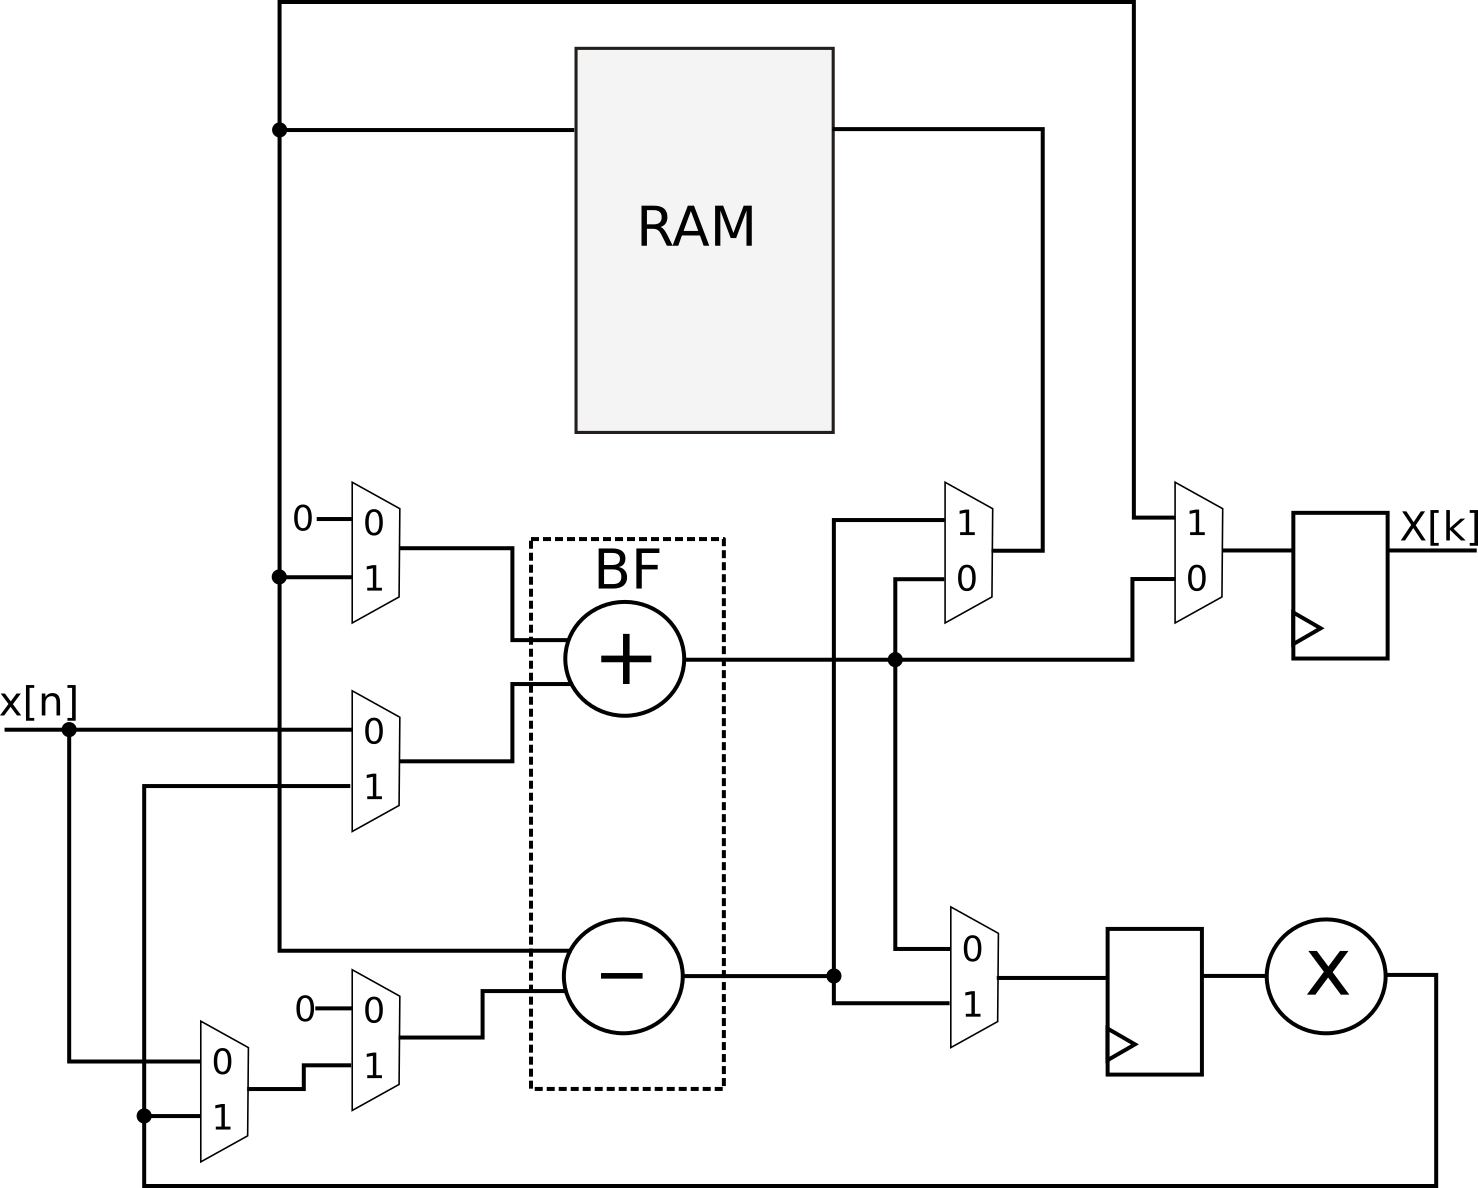
\includegraphics[width=10cm]{./figures/datapath.png}
        \caption{Esquema del datapath de la arquitectura radix-2}
        \label{fig:datapath}
\end{figure}

A través de los multiplexores se configura el \textit{datapath} de acuerdo a la etapa en que se encuentra y
el tipo de operación a realizar. De la figura \ref{fig:radix2blocks} se deduce que en cada fase de
cómputo se puede realizar una de dos acciones posibles, entra un dato a memoria mientras que otro dato 
sale de memoria hacia el multiplicador o se opera en el \textit{butterfly} con un dato de memoria y otro dato que viene
de la entrada o de la etapa anterior.

En la figura \ref{fig:datapathMem} se muestran las tres configuraciones posibles del \textit{datapath} para
las operaciones de tranferencias de datos en memoria. En este tipo de operación se lee un dato de
memoria y se envía al multiplicador para realizar el producto por el \textit{twiddle fator} o hacia
la salida y se escribe un dato en memoria proveniente de la entrada o de la etapa anterior a través
del \textit{delay register}.

% \begin{figure}[htb!]
%         \centering
%         \subfigure[Etapa
%         inicial]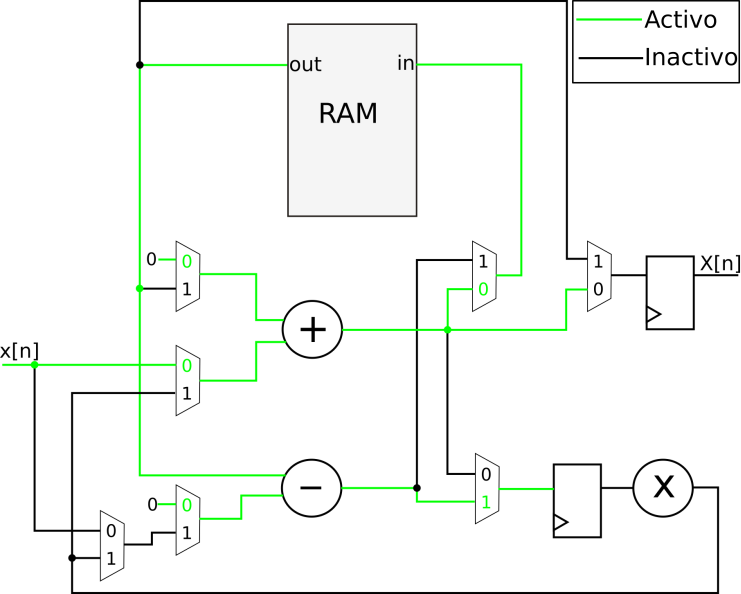
\includegraphics[width=7cm]{./figures/datapath_mem1.png}}
%         \subfigure[Etapas
%         intermedias]}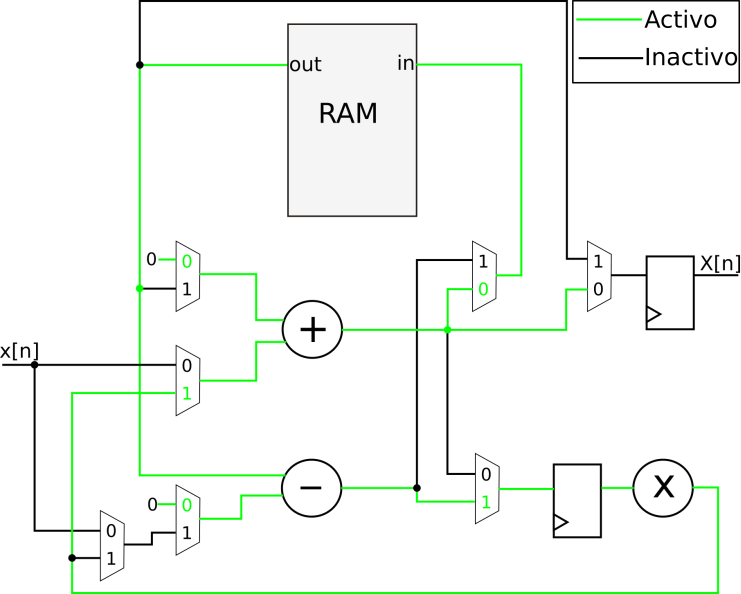
\includegraphics[width=7cm]{./figures/datapath_memint.png}}
%         \subfigure[Etapa
%         final]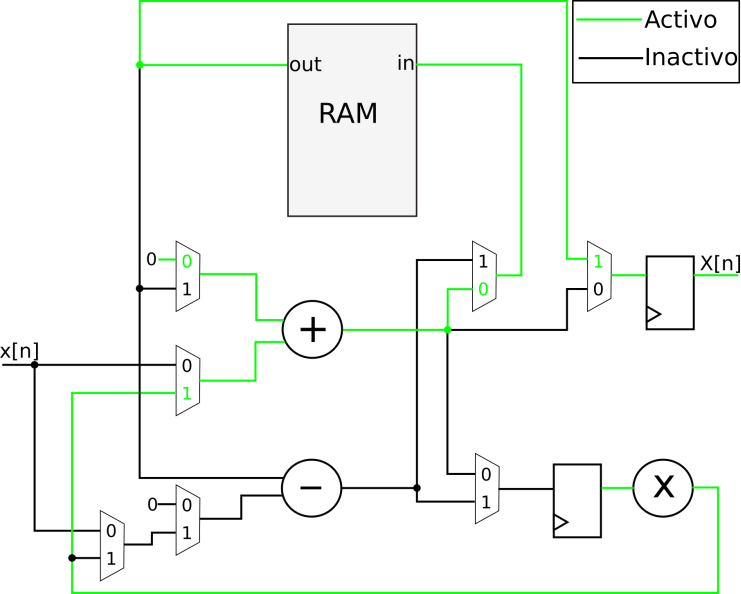
\includegraphics[width=7cm]{./figures/datapath_memf.png}}
%         \caption{Datapath para operaciones de transferencia en memoria}
%         \label{fig:datapathMem}
% \end{figure}

\begin{figure}[htb!]
        \centering
        \begin{subfigure}{\columnwidth}\centering
        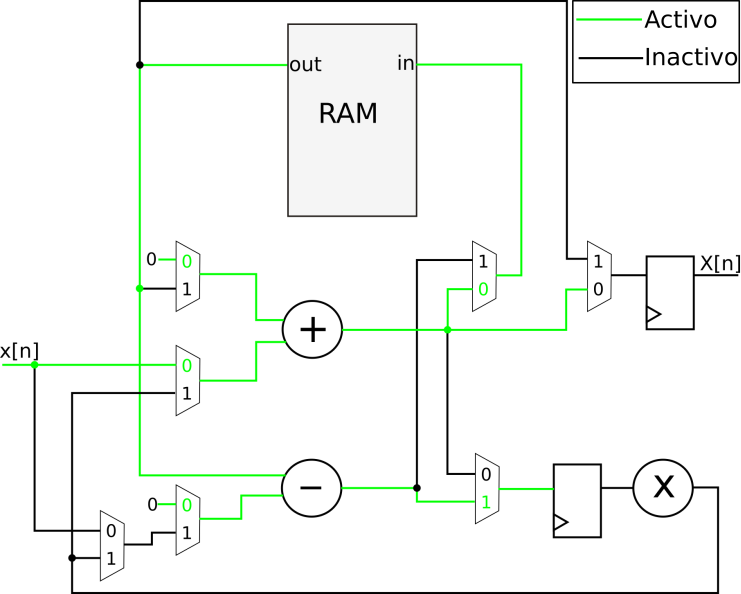
\includegraphics[width=7cm]{./figures/datapath_mem1.png}
        \caption{Etapa inicial}
        \end{subfigure}
        \begin{subfigure}{\columnwidth}\centering
        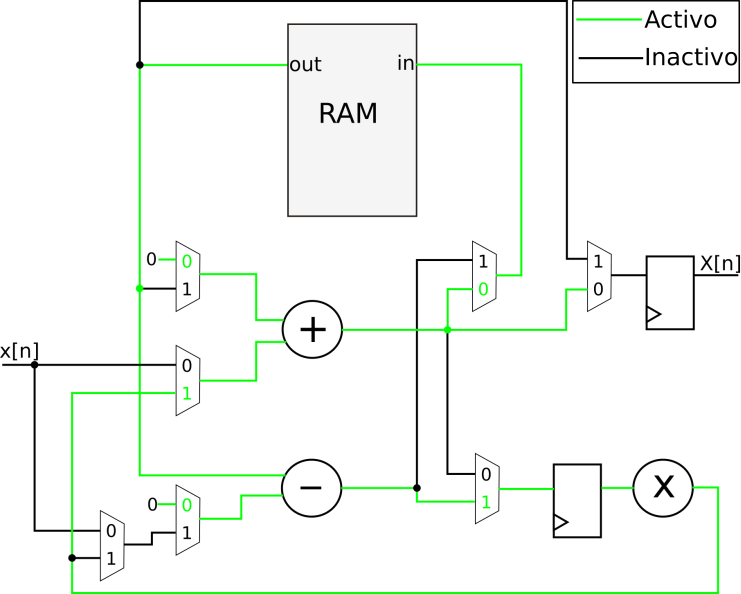
\includegraphics[width=7cm]{./figures/datapath_memint.png}
        \caption{Etapas intermedias}
        \end{subfigure}
        \begin{subfigure}{\columnwidth}\centering
        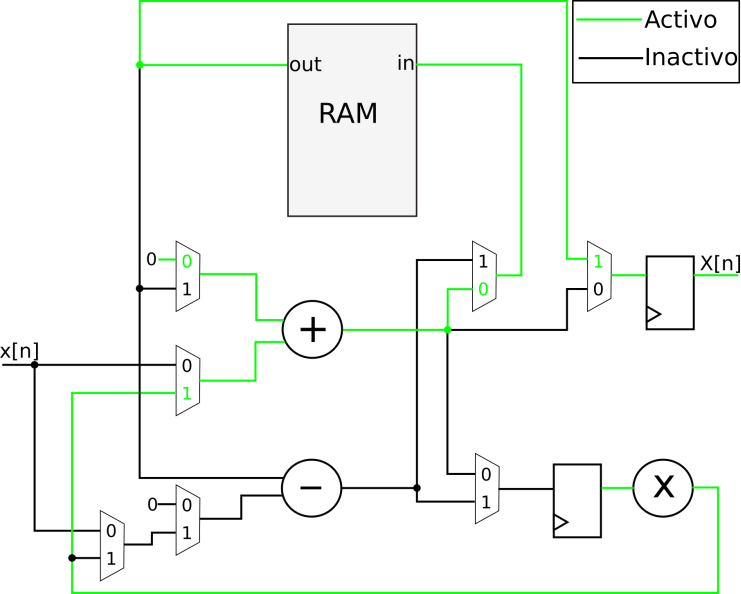
\includegraphics[width=7cm]{./figures/datapath_memf.png}
        \caption{Etapa final}
        \end{subfigure}
        \caption{Datapath para operaciones de transferencia en memoria}
        \label{fig:datapathMem}
\end{figure}

En la figura \ref{fig:datapathBut} se muestran los posibles \textit{datapath} para las operaciones en el
butterfly. Dependiendo de si la etapa es la etapa inicial o una intermedia uno de los operandos será
la entrada de la arquitectura o un dato de la entrada anterior almacenado en el \textit{delay
register} y el otro operando provendrá de la memoria. La salida del restador del butterfly se envía
directamente a memoria y la salida del sumador puede ir al \textit{delay register} para ser
utilizado en la etapa siguiente o puede ser direccionado a la salida de la arquitectura dependiendo
de si la etapa es intermedia o es la etapa de salida.

\begin{figure}[htb!]
        \centering
        \begin{subfigure}{\columnwidth}\centering
        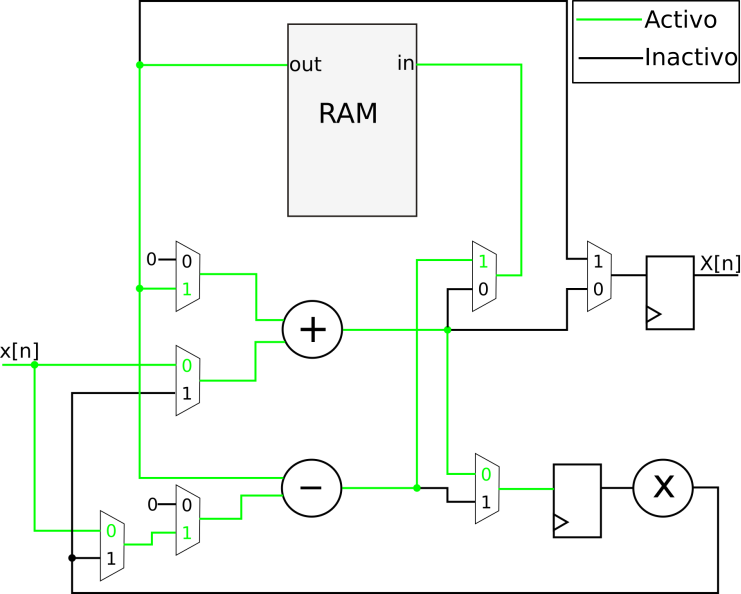
\includegraphics[width=7cm]{./figures/datapath_but1.png}
        \caption{Etapa inicial}
        \end{subfigure}
        \begin{subfigure}{\columnwidth}\centering
        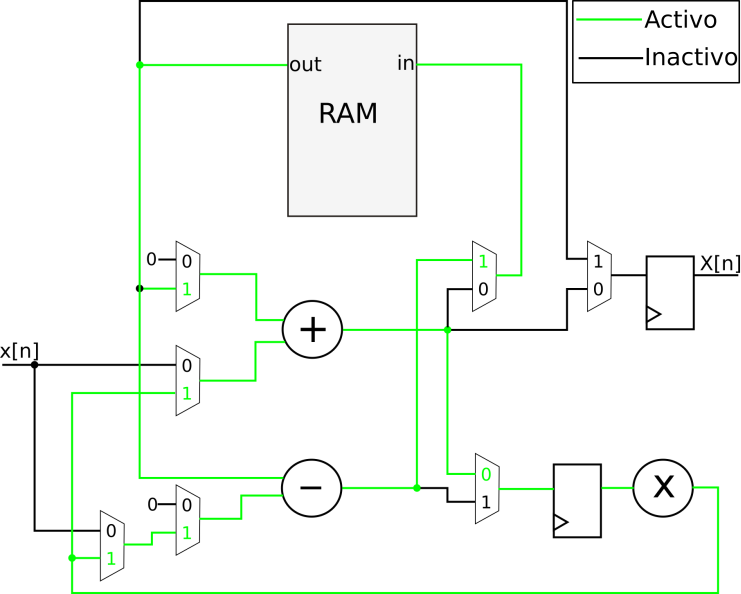
\includegraphics[width=7cm]{./figures/datapath_butint.png}
        \caption{Etapas intermedias}
        \end{subfigure}
        \begin{subfigure}{\columnwidth}\centering
        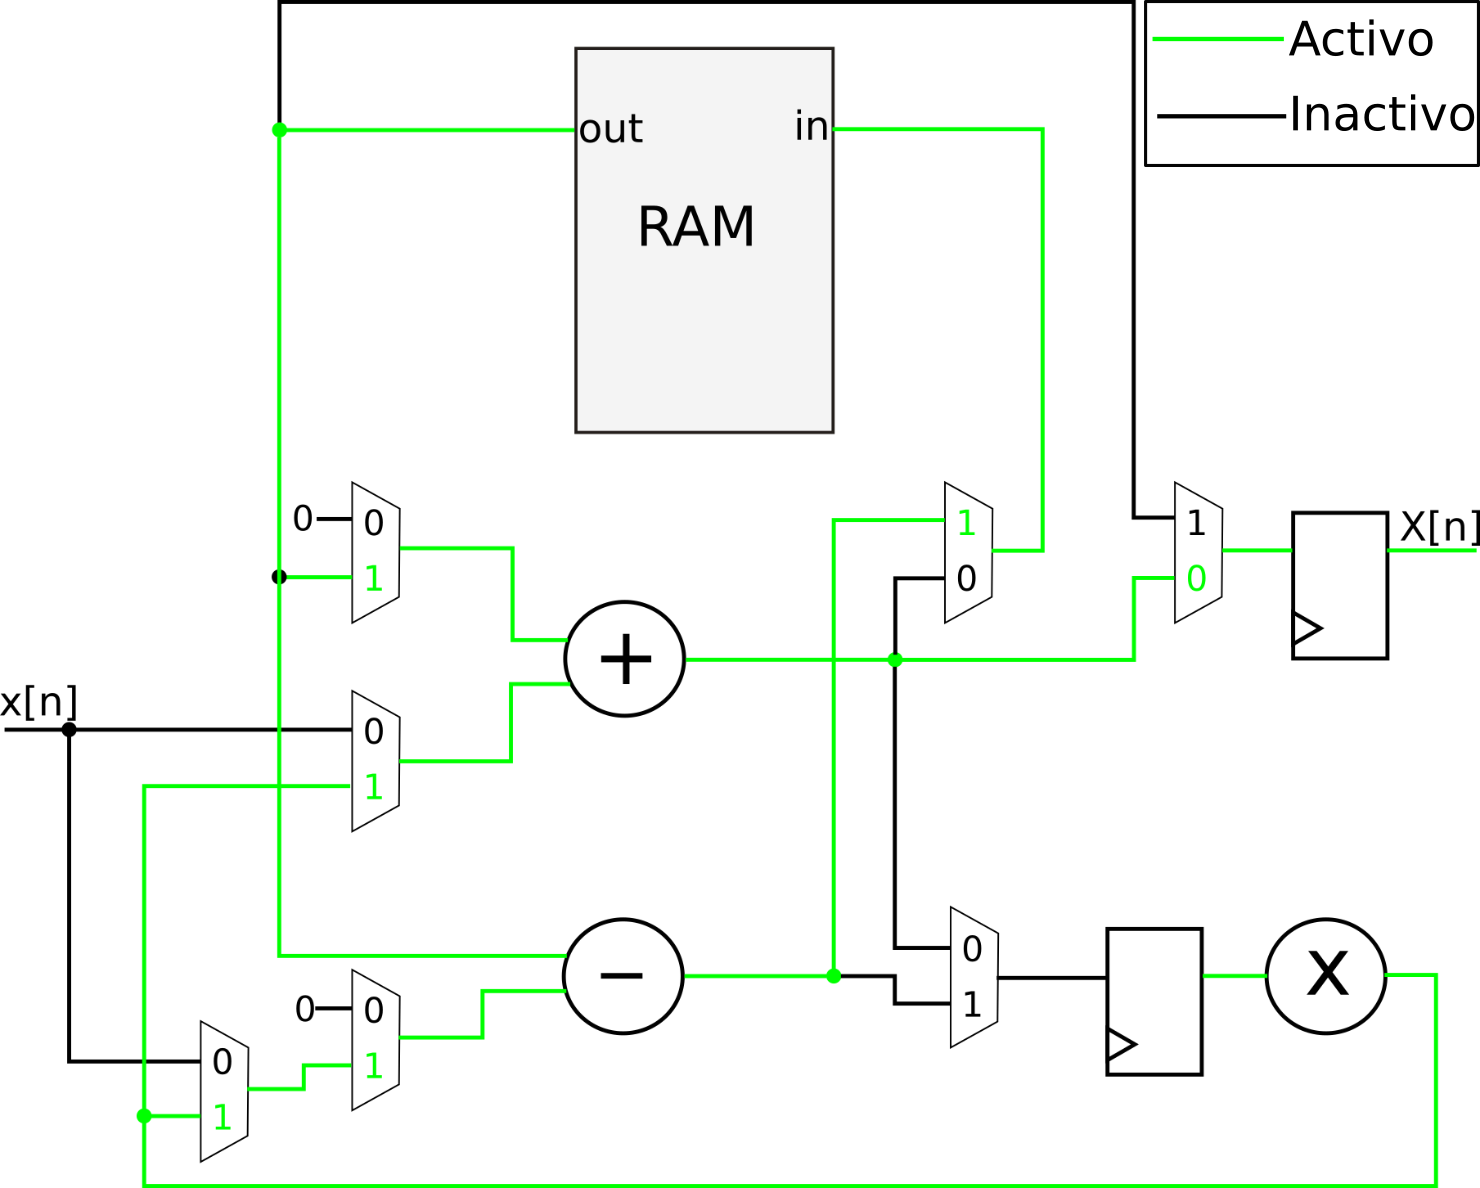
\includegraphics[width=7cm]{./figures/datapath_butf.png}
        \caption{Etapa final}
        \end{subfigure}
        \caption{Datapath para operaciones en butterfly}
        \label{fig:datapathBut}
\end{figure}

\subsection{Unidad de control}

La unidad de control debe contener la máquina de estados que controla el funcionamiento de la
arquitectura, la configuración del \textit{datapath} en cada ciclo de \textit{clock}, el manejo de
la memoria donde se almacenan los valores de cálculo y la generación de los \textit{twiddle factors}
para el multiplicador.

Teniendo en cuenta que ingresa a la arquitectura un punto nuevo cada $log_2(N)$ ciclos de
\textit{clock} se utiliza un contador de etapas de longitud $log_2(log_2(N))$ para identificar la
etapa del cómputo de la fft en que se encuentra la arquitectura. El desborde de este contador
alimenta otro contador de longitud  $log_2(N)$ que cuenta la cantidad de puntos que han ingresado a
la arquitectura. Con estos dos contadores se lleva el control de la máquina de estados, que controla
la configuración del \textit{datapath} y la memoria, y la generación de los \textit{twiddle
factors}.

En la subsección \ref{sec:datapath} se describieron las distintas configuraciones del \textit{datapath}, que
deben ser gestionadas por la unidad de control de acuerdo a la etapa en que se encuentra la
arquitectura y si debe realizar una transferencia a memoria o un cálculo en el butterfly. Tomando
como ejemplo la radix-2 de $8$ puntos de la figura \ref{fig:r2_8_c3}, se ve que en la primera etapa se debe esperar la llegada del quinto punto para realizar una operación en el \textit{butterfly}, por lo que las primeras cuatro operaciones de esa etapa serán trasnferencias de los puntos a memoria y las últimas cuatro serán operaciones en el
\textit{butterfly}. Para la segunda etapa la secuencia será de dos operaciones de transferencia a
memoria y dos de operaciones aritméticas. Y para la última etapa serán operaciones de transferencia
a memoria y aritméticas alternadas de a una. Entonces para una cierta etapa $i \epsilon \{0 \leq i
\leq log_2(N)-1\}$ la cantidad de operaciones consecutivas de cada tipo está dada por

\begin{equation}
log_2(\frac{N}{i+1})
\label{eq:etapas}
\end{equation}

Para determinar si se debe realizar una transferencia a memoria o una operación aritmética, se
utiliza un solo bit del contador de puntos. El bit a evaluar se determina en función de la etapa que
se está procesando, a través del \textit{stg\_ctr}, el contador de etapas, de $\log_2(\log_2(N))$
bits, como se muestra en la figura \ref{fig:r2conts}.

% Para determinar \ref{eq:etapas} en cada ciclo de \textit{clock} se observa en el contador de puntos
% el bit dado por $log_2(N) - contador_{etapas} - 1$, entonces en la primer etapa (contador de etapas
% en cero) se evalúa el bit más alto del contador de puntos, y así sucesivamente hasta evaluar el bit
% más bajo del contador de puntos en la última etapa (donde $contador_{etapas} = log_2(N) - 1$). En
% la figura \ref{fig:r2conts} se muestra un esquema de la selección del bit del contador de puntos
% de acuerdo al valor del $contador_{etapas}$ para una arquitectura de 256 puntos. De esta forma si el
% bit del contador de puntos correspondiente a una etapa vale $'0'$ se realiza una trasnferencia a
% memoria, y si vale $'1'$ se realiza una operación en el \textit{butterfly}.

\begin{figure}[htb!]
        \centering
        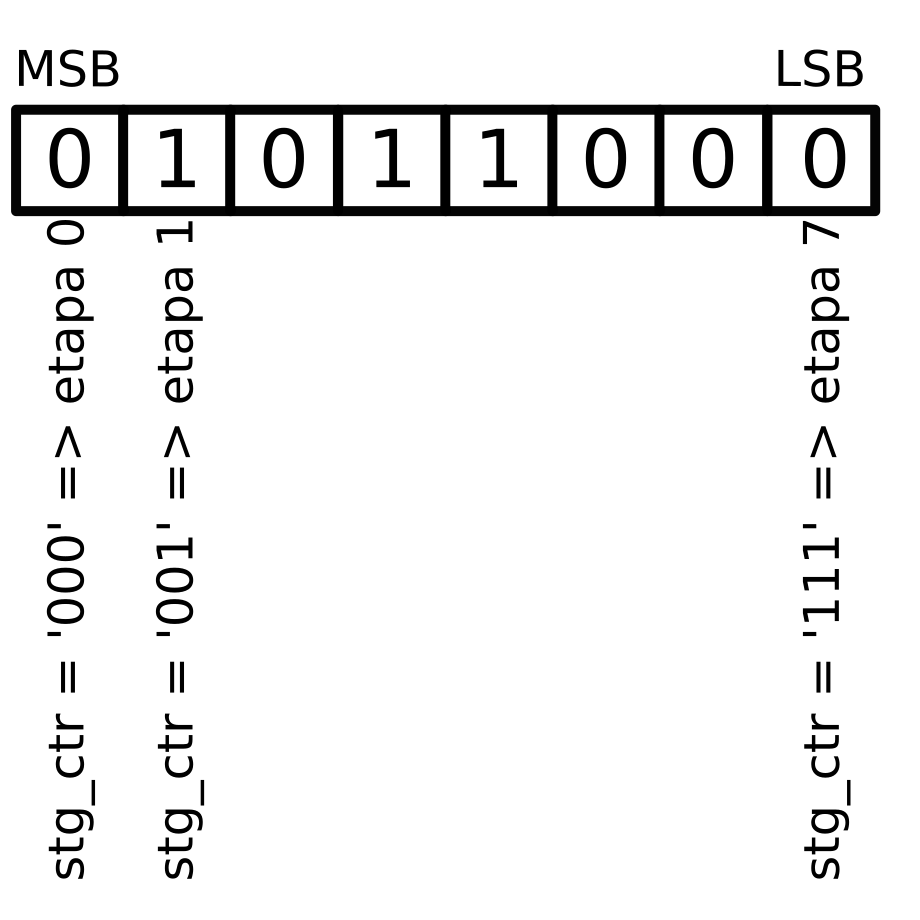
\includegraphics[width=6cm]{./figures/r2conts.png}
        \caption{Selección del bit del contador de puntos a evaluar}
        \label{fig:r2conts}
\end{figure}


\subsubsection{Máquinas de estados}

La unidad de control se compone de una máquina de estados principal que controla la inicialización
de los módulos de la arquitectura y una máquina de estados operativa que controla la
configuración del \textit{datapath} dependiendo de la operación que se debe realizar.
En la figura \ref{fig:mainSMr2} se muestran los estados y transiciones de la máquina de estados
principal.

\begin{figure}[htb!]
        \centering
        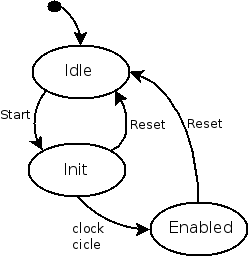
\includegraphics[width=6cm]{./figures/SMr2gen.png}
        \caption{Estados de la máquina de estados principial}
        \label{fig:mainSMr2}
\end{figure}

El estado inicial de la arquitectura es el estado
\textit{Idle}, donde permanece aguardando una señal para iniciar el proceso. La señal de
\textit{start} tiene la finalidad de sincronizar la arquitectura con el entorno al que está conectada, y lleva la
máquina de estados al estado \textit{Init} donde se inicializan los registros a valores conocidos y
se configura el \textit{datapath} para comenzar el procesamiento, leyendo ya el primer dato de la
entrada. Un ciclo de \textit{clock} después la máquina de estados pasa directamente al estado \textit{Enabled} 
donde se realiza el procesamiento. Dentro de
este estado se encuentra la máquina de estados operativa que se describe a continuación.

\begin{figure}[htb!]
        \centering
        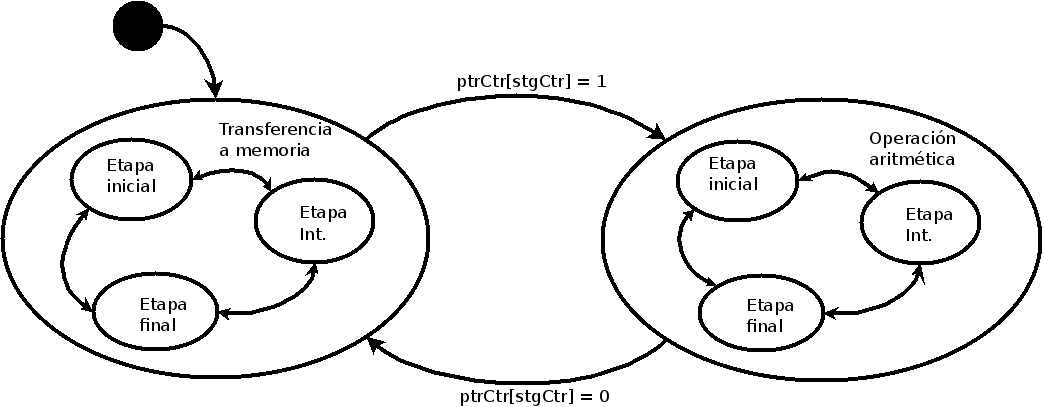
\includegraphics[width=13cm]{./figures/SMr2op.png}
        \caption{Máquina de estados operativa para modo \textit{enabled}}
        \label{fig:opSMr2}
\end{figure}

En la figura \ref{fig:opSMr2} se observan los estados y transiciones de la máquina de estados
que controla la configuración del \textit{datapath} de acuerdo al tipo de operación a
realizar.
En cada uno de los estados principales funciona una máquina de estados secundaria que realiza
ajustes menores de acuerdo a si la etapa actual es la etapa inicial, una intermedia o la etapa final. $ptrCtr[stgCtr]$ hace
referencia al bit del contador de puntos correspondiente al valor del contador de etapas, de
acuerdo a lo expuesto en la figura \ref{fig:r2conts}.\\
Esta máquina de estados controla además la señal de habilitación de escalamiento para la etapa
actual de acuerdo al vector de escalamiento de entrada a la arquitectura. También controla, a través
del contador de puntos y el de etapas, las señales de \textit{handshaking} de salida, indicando si
el dato de salida es un dato válido, señal \textit{data\_valid} y las señales que indican si es el
punto inicial (\textit{soo}) o final (\textit{done})del cómputo actual.

\subsubsection{Control de la memoria}

Dado que el algoritmo radix-2 permite el alojamiento \textit{data in place} el manejo de la memoria
es relativamente sencillo. 
En cada operación de una etapa se realiza siempre una escritura de datos, ya sea un dato entrante a
la etapa (nuevo o de una etapa anterior) o del resultado de una operación aritmética. En cambio solo
se realizan lecturas de memoria en las etapas intermedias y en la última.
Al ser un algoritmo \textit{data in place} las direcciones de memoria tanto de escritura como de
lectura se calculan utilizando el contador de puntos, ya que cada en cada posición de memoria
donde se alojaba un dato utilizado para una operación aritmética se alojará el resultado
correspondiente a esa operación una vez realizada. Entonces en una etapa determinada se lee la
posición de memoria $k$, se realiza un cálculo con ese dato, y se guarda nuevamente en la posición
$k$ el resultado del cálculo.
Al acceder continuamente a la memoria tanto en modo escritura como lectura, las señales
correspondientes de control de la memoria están siempre en modo habilitación.

\subsubsection{Control del datapath}

El control del \textit{datapath} se realiza mediante los multiplexores que se ven en la figura
\ref{fig:datapath} a través de señales digitales. En cada ciclo de \textit{clock}, de acuerdo a la máquina de
estados que decide en que etapa se encuentra el algoritmo y dependiendo de la operación a realizar
se configuran los multiplexores para conformar el datapath según las figuras \ref{fig:datapathMem}
y \ref{fig:datapathBut}.

\subsection{Integración de la unidad de control}

En la figura \ref{fig:datapathmem} se muestra el \textit{datapath} de la figura \ref{fig:datapath} con el
agregado de las señales de control sobre cada módulo. No se muestra la unidad de control en forma
explícita para mantener la claridad del esquema. En el bloque butterfly además del
sumador/restador se integra el algoritmo de escalamiento que se describe en la sección
\ref{sec:secEscal}.

\begin{figure}[htb!]
        \centering
        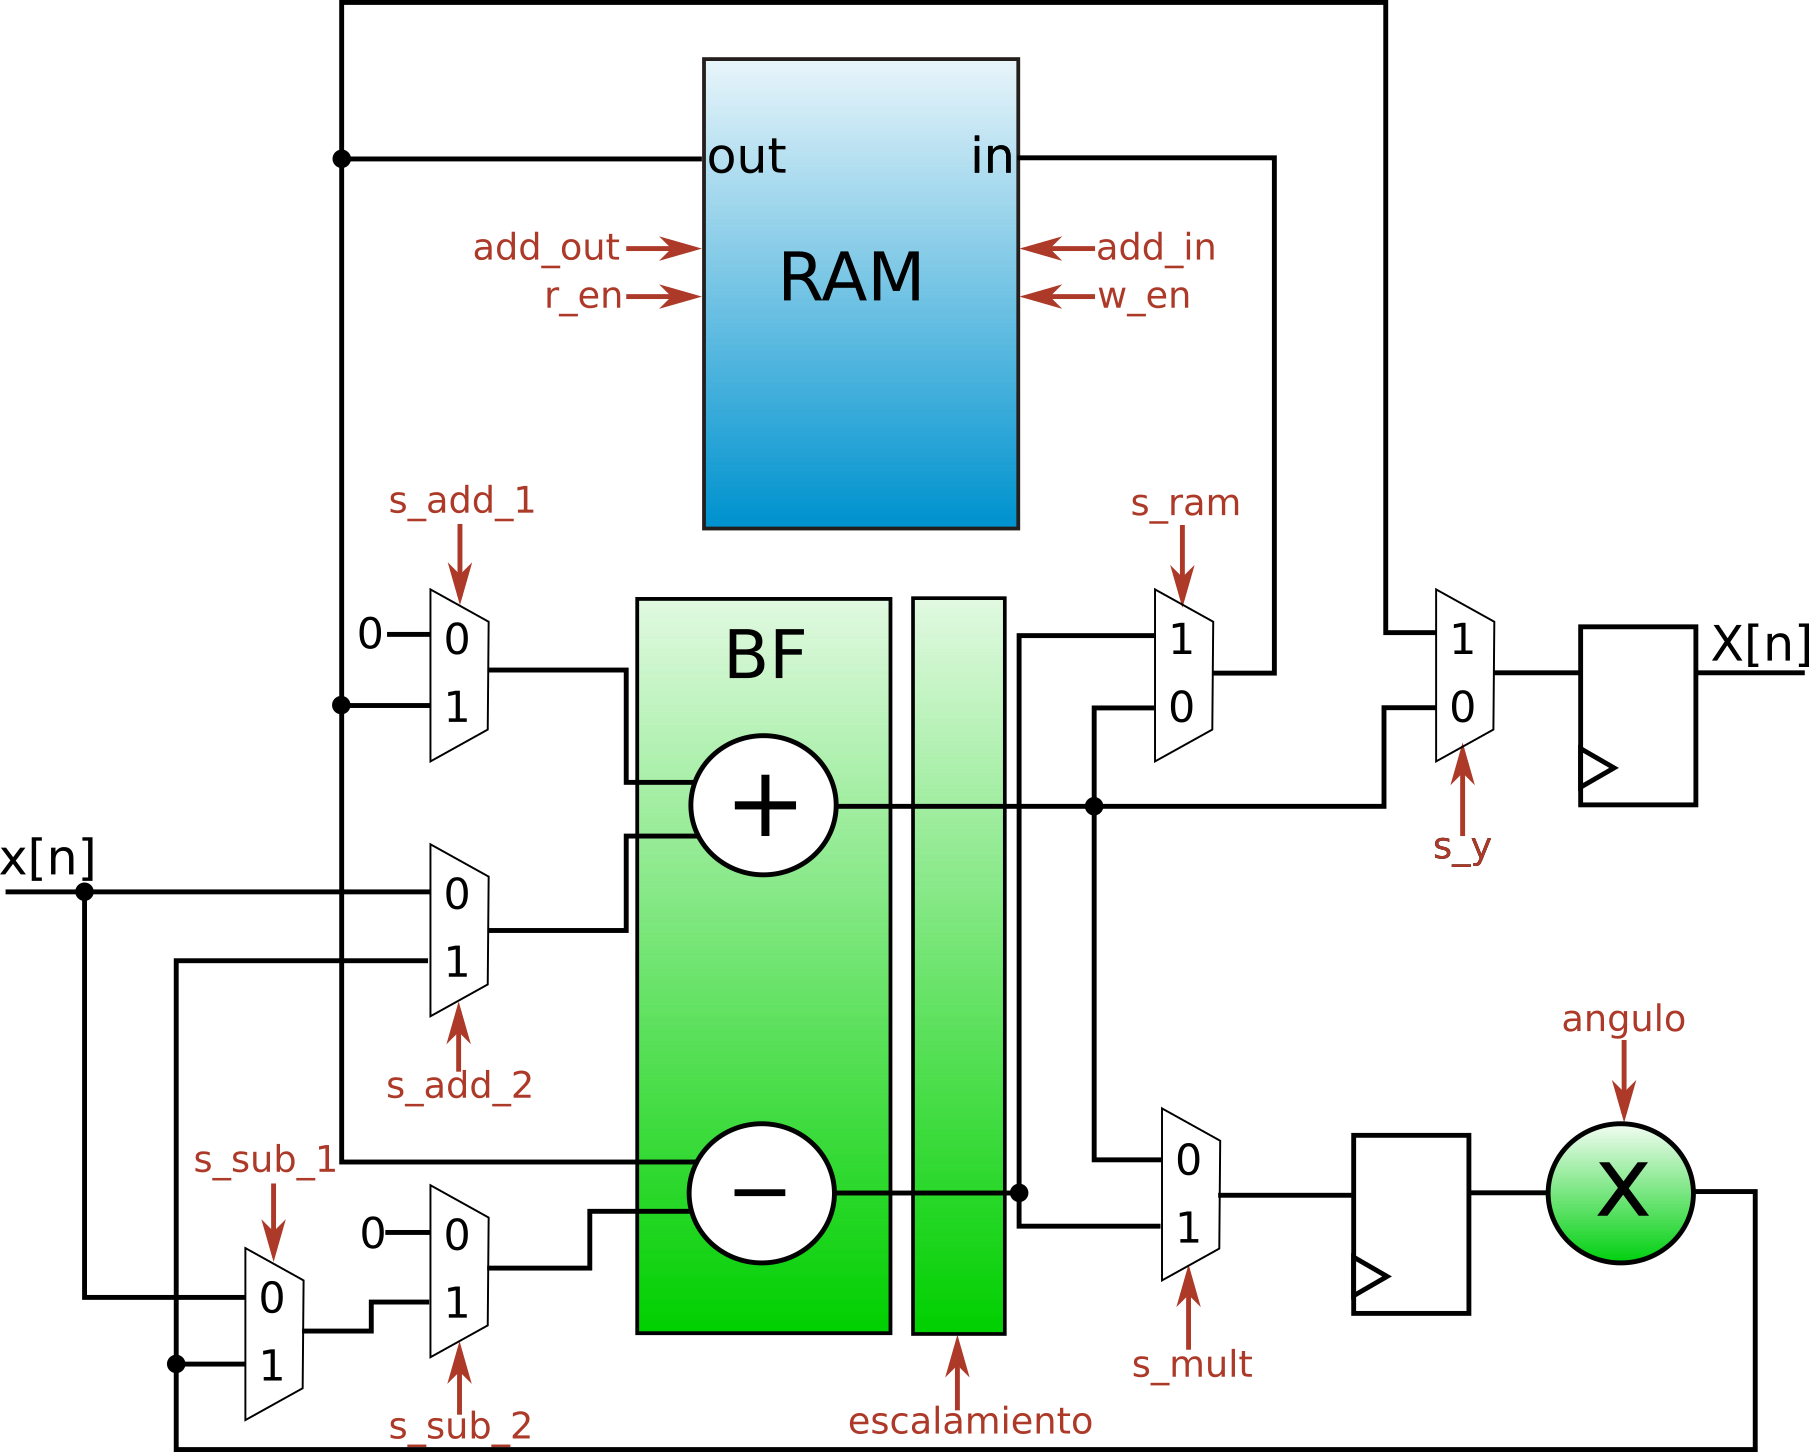
\includegraphics[width=12cm]{./figures/datapathMem.png}
        \caption{Datapath con las señales de control}
        \label{fig:datapathmem}
\end{figure}

En la figura \ref{fig:datapathmem} se muestran las siguientes señales de control (se indica entre
paréntesis el tamaño de las señales en caso que sea mayor a 1):

\begin{itemize}
  \item \textbf{add\_in} ($log_2(N)$) \textit{address in}, dirección de memoria donde se escribirá
  el dato
  \item \textbf{w\_en} \textit{write enable}, señal de habilitación de escritura en memoria
  \item \textbf{add\_out} ($log_2(N)$) \textit{address out}, dirección de memoria desde la que leerá
  el dato
  \item \textbf{r\_en} \textit{read enable}, señal de habilitacón de lectura de memoria
  \item \textbf{s\_add\_1} señal de control del multiplexor de la entrada $1$ del sumador
  \item \textbf{s\_add\_2} señal de control del multiplexor de la entrada $2$ del sumador
  \item \textbf{s\_sub\_1} señal de control del multiplexor de tipo de entrada del restador
  \item \textbf{s\_sub\_2} señal de control del multiplexor de entrada del restador
  \item \textbf{s\_mult} señal de control del multiplexor de entrada del multiplicador
  \item \textbf{s\_ram} señal de control del multiplexor de entrada de la memoria RAM
  \item \textbf{s\_y} señal de control del multiplexor de origen de la salida
  \item \textbf{angulo} ($N+1$) angulo de rotación para el multiplicador, ya sea cordic o
  multiplicador complejo.
  \item \textbf{escalamiento} señal de indicación de que en la etapa actual se realiza
  redondeo/truncamiento. 
\end{itemize}

\section{Arquitectura Radix-4}
\subsection{Descripción general}

El algoritmo Radix-4 descompone el cómputo de una DFT de N puntos en $\nu$ DFTs de 4 puntos cada
una de forma que $N = 4^\nu$.\\ Partiendo de la definición de DFT:

\begin{equation}
\begin{split}
 X_k &= \sum\limits_{n=0}^{N-1}x_n W_N^{kn} \\
 &= \sum\limits_{n=0}^{\frac{N}{4}-1}x_n W_N^{kn} + \sum\limits_{n=\frac{N}{4}}^{\frac{N}{2}-1}x_n
 W_N^{kn} + \sum\limits_{n=\frac{N}{2}}^{\frac{3N}{4}-1}x_n W_N^{kn} +
 \sum\limits_{n=\frac{3N}{4}}^{N-1}x_n W_N^{kn} \\
 &= \sum\limits_{n=0}^{\frac{N}{4}-1}x_n W_N^{kn} +
 \sum\limits_{n=0}^{\frac{N}{4}-1}x_{n+\frac{N}{4}} W_N^{k(n+\frac{N}{4})} +
 \sum\limits_{n=0}^{\frac{N}{4}-1}x_{n+\frac{N}{2}} W_N^{k(n+\frac{N}{2})} + 
 \sum\limits_{n=0}^{\frac{N}{4}-1}x_{n+\frac{3N}{4}} W_N^{k(n+\frac{3N}{4})} \\
 &= \sum\limits_{n=0}^{\frac{N}{4}-1}x_n W_N^{kn} +
 W_4^k \sum\limits_{n=0}^{\frac{N}{4}-1}x_{n+\frac{N}{4}} W_N^{kn} +
 W_4^{2k} \sum\limits_{n=0}^{\frac{N}{4}-1}x_{n+\frac{N}{2}} W_N^{kn} + 
 W_4^{3k}\sum\limits_{n=0}^{\frac{N}{4}-1}x_{n+\frac{3N}{4}} W_N^{kn} \\
 &= \sum\limits_{n=0}^{\frac{N}{4}-1}(x_n + x_{n+\frac{N}{4}} W_4^k + x_{n+\frac{N}{2}} W_4^{2k} + 
 x_{n+\frac{3N}{4}} W_4^{3k}) W_N^{kn}
\end{split}
\label{eq:radix4_1}
\end{equation}

El resultado final en (\ref{eq:radix4_1}) se puede descomponer en cuatro subproblemas para los casos
$4k$, $4k+1$, $4k+2$ y $4k+3$ dando lugar a:

\begin{equation}
\begin{split}
Y_k = X_{4k} &= \sum\limits_{n=0}^{\frac{N}{4}-1}(x_n + x_{n+\frac{N}{4}} W_4^{4k} +
x_{n+\frac{N}{2}} W_4^{2*4k} + x_{n+\frac{3N}{4}} W_4^{3*4k}) W_N^{4kn} \\
&= \sum\limits_{n=0}^{\frac{N}{4}-1}(x_n + x_{n+\frac{N}{4}} + x_{n+\frac{N}{2}} +
x_{n+\frac{3N}{4}}) W_{\frac{N}{4}}^{kn} \\
&= \sum\limits_{n=0}^{\frac{N}{4}-1} y_k W_{\frac{N}{4}}^{kn}, \qquad k = 0,1,\ldots,\frac{N}{4}-1
\end{split}
\label{eq:radix4_Y}
\end{equation}

\begin{equation}
\begin{split}
Z_k = X_{4k+1} &= \sum\limits_{n=0}^{\frac{N}{4}-1}(x_n + x_{n+\frac{N}{4}} W_4^{4k+1} +
x_{n+\frac{N}{2}} W_4^{2*(4k+1)} + x_{n+\frac{3N}{4}} W_4^{3*(4k+1)}) W_N^{(4k+1)n} \\
&= \sum\limits_{n=0}^{\frac{N}{4}-1}((x_n - x_{n+\frac{N}{2}}) -j (x_{n+\frac{N}{4}}
-x_{n+\frac{3N}{4}})) W_N^{k} W_{\frac{N}{4}}^{kn} \\
&= \sum\limits_{n=0}^{\frac{N}{4}-1} z_k W_{\frac{N}{4}}^{kn}, \qquad k = 0,1,\ldots,\frac{N}{4}-1
\end{split}
\label{eq:radix4_Z}
\end{equation}

\begin{equation}
\begin{split}
G_k = X_{4k+2} &= \sum\limits_{n=0}^{\frac{N}{4}-1}(x_n + x_{n+\frac{N}{4}} W_4^{4k+2} +
x_{n+\frac{N}{2}} W_4^{2*(4k+2)} + x_{n+\frac{3N}{4}} W_4^{3*(4k+2)}) W_N^{(4k+2)n} \\
&= \sum\limits_{n=0}^{\frac{N}{4}-1}((x_n + x_{n+\frac{N}{2}}) - (x_{n+\frac{N}{4}}
+ x_{n+\frac{3N}{4}})) W_N^{2k} W_{\frac{N}{4}}^{kn} \\
&= \sum\limits_{n=0}^{\frac{N}{4}-1} g_k W_{\frac{N}{4}}^{kn}, \qquad k = 0,1,\ldots,\frac{N}{4}-1
\end{split}
\label{eq:radix4_G}
\end{equation}

\begin{equation}
\begin{split}
H_k = X_{4k+3} &= \sum\limits_{n=0}^{\frac{N}{4}-1}(x_n + x_{n+\frac{N}{4}} W_4^{4k+3} +
x_{n+\frac{N}{2}} W_4^{2*(4k+3)} + x_{n+\frac{3N}{4}} W_4^{3*(4k+3)}) W_N^{(4k+3)n} \\
&= \sum\limits_{n=0}^{\frac{N}{4}-1}((x_n - x_{n+\frac{N}{2}}) +j (x_{n+\frac{N}{4}}
- x_{n+\frac{3N}{4}})) W_N^{3k} W_{\frac{N}{4}}^{kn} \\
&= \sum\limits_{n=0}^{\frac{N}{4}-1} h_k W_{\frac{N}{4}}^{kn}, \qquad k = 0,1,\ldots,\frac{N}{4}-1
\end{split}
\label{eq:radix4_H}
\end{equation}

Entonces, la unidad aritmética de la arquitectura radix-4 debe procesar cuatro puntos, $x_n$,
$x_{n+\frac{l}{4}}$, $x_{n+\frac{l}{2}}$ y $x_{n+\frac{l}{4}}$, obteniéndose como resultado:

\begin{equation}
y_n = (x_n + x_{n+\frac{l}{4}} + x_{n+\frac{l}{2}} + x_{n+\frac{3l}{4}}) \qquad k =
0,1,\ldots,\frac{N}{4}-1
\label{eq:radix4_suby}
\end{equation}

\begin{equation}
z_n = ((x_n - x_{n+\frac{l}{2}}) -j (x_{n+\frac{l}{4}}
-x_{n+\frac{3l}{4}})) W_N^{k} \qquad k = 0,1,\ldots,\frac{N}{4}-1
\label{eq:radix4_subz}
\end{equation}

\begin{equation}
g_n = ((x_n + x_{n+\frac{l}{2}}) - (x_{n+\frac{l}{4}}
+ x_{n+\frac{3l}{4}})) W_N^{2k} \qquad k = 0,1,\ldots,\frac{N}{4}-1
\label{eq:radix4_subg}
\end{equation}

\begin{equation}
h_n = ((x_n - x_{n+\frac{l}{2}}) +j (x_{n+\frac{l}{4}} - x_{n+\frac{3l}{4}})) W_N^{3k} \qquad k = 0,1,\ldots,\frac{N}{4}-1
\label{eq:radix4_subh}
\end{equation}

donde $l$ depende de la etapa del cómputo a la que pertenece el cálculo y se define como sigue

\begin{equation}
\begin{split}
l_1 &= N \\
l_2 &= \log_4(N) \\
l_3 &= \log_4(\log_4(N))\\ 
..&.\\
l_\nu &= 4
\end{split}
\label{eq:radix_4_arit_l}
\end{equation}

donde $l_i$ corresponde a la etapa i-ésima de una FFT de $N=4^\nu$ puntos.

En la figura \ref{fig:r4_diag} se muestra un esquema del cómputo de una radix-4 para 16 puntos,
similar al esquema de la radix-2 de la figura \ref{fig:r2_8_c3}, donde se ve el cómputo aritmético
utilizando cuatro puntos como entrada y obteniendo cuatro puntos como salida.

\begin{figure}[htb!]
        \centering
        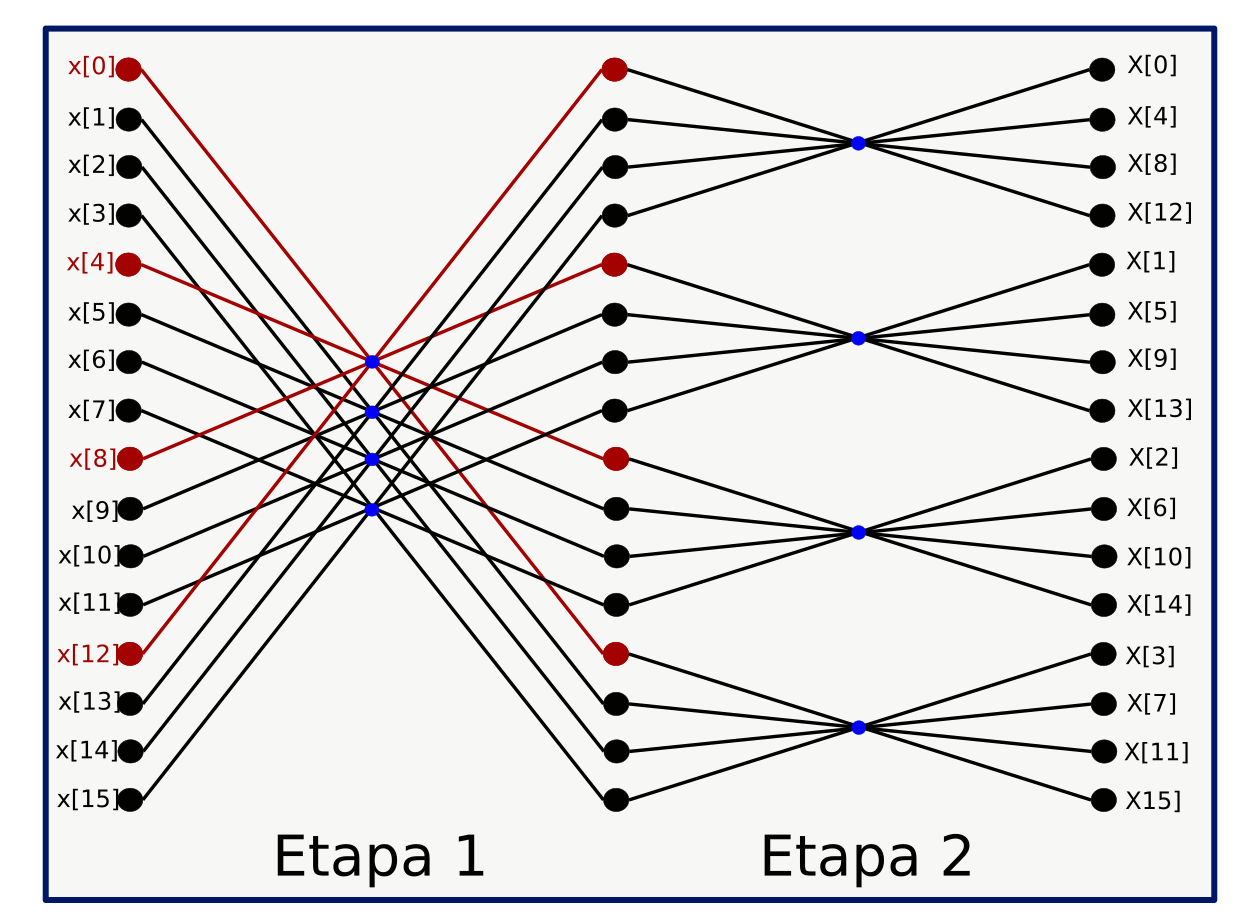
\includegraphics[width=10cm]{./figures/r4_16.png}
        \caption{Esquema de una FFT radix-4 de 16 puntos}
        \label{fig:r4_diag}
\end{figure}

Este funcionamiento implica que para realizar un cálculo aritmético se deben tener almacenados en
memoria tres puntos, que deben ser extraídos de memoria al entrar el cuarto punto para realizar el
cálculo. Luego del cálculo se obtienen cuatro puntos de los cuales tres son almacenados en memoria
mientras que el cuarto punto es utilizado en la etapa siguiente.


En la figura \ref{fig:radix4blocks} se muestra un diagrama en bloques simplificado de la
arquitectura radix-4 iterativa. Se diferencian claramente tres partes, la memoria, de tres entradas
y tres salidas, la unidad aritmética conformada por el \textit{dragonfly} (nombre que se le asigna
al sumador/restados cuádruple que realiza las operaciones en la radix-4), el multiplicador, y la
unidad de control. 
Esta arquitectura presenta un nivel superior de complejidad que la radix-2 que se traduce
principalmente en una unidad de control más compleja y la unidad aritmética que puede ser un poco
más lenta reduciendo así la frecuencia máxima de trabajo. Pero a su vez ofrece la ventaja de
requerir la mitad de etapas que la radix-2 para realizar el cómputo de una FFT de la misma cantidad 
de puntos.

\begin{figure}[htb!]
        \centering
        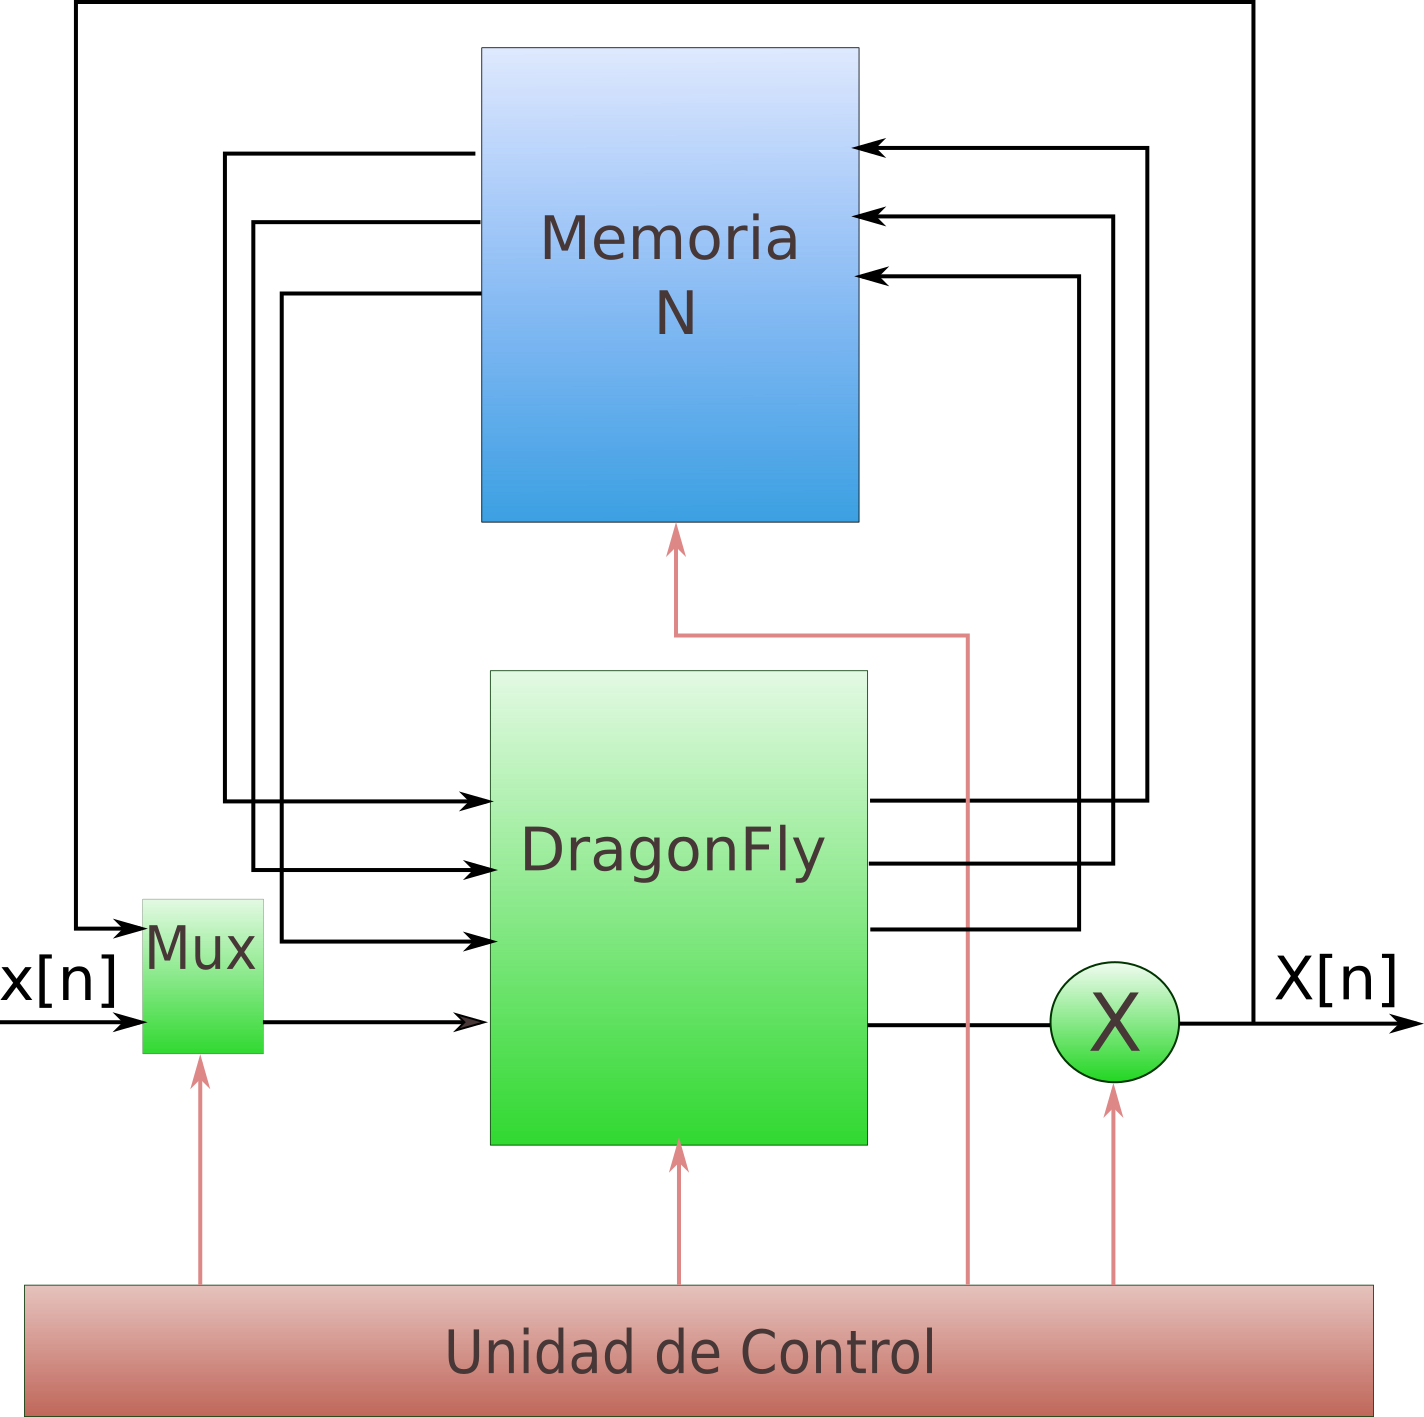
\includegraphics[width=10cm]{./figures/radix4blocks.png}
        \caption{Diagrama simplificado de la arquitectura radix-4 iterativa}
        \label{fig:radix4blocks}
\end{figure}

\subsection{Memoria} \label{sec:r4mem}

Como se explicó, en la arquitectura radix-4 se deben escribir y leer de memoria tres puntos en forma
simultánea cada vez que se realiza una operación aritmética.
En la figura \ref{fig:tripleRam} se presenta el bloque de memoria RAM de triple entrada y triple
salida con sus puertos de conexión. Los valores entre corchetes indican el tamaño del bus
correspondiente.

\begin{figure}[htb!]
        \centering
        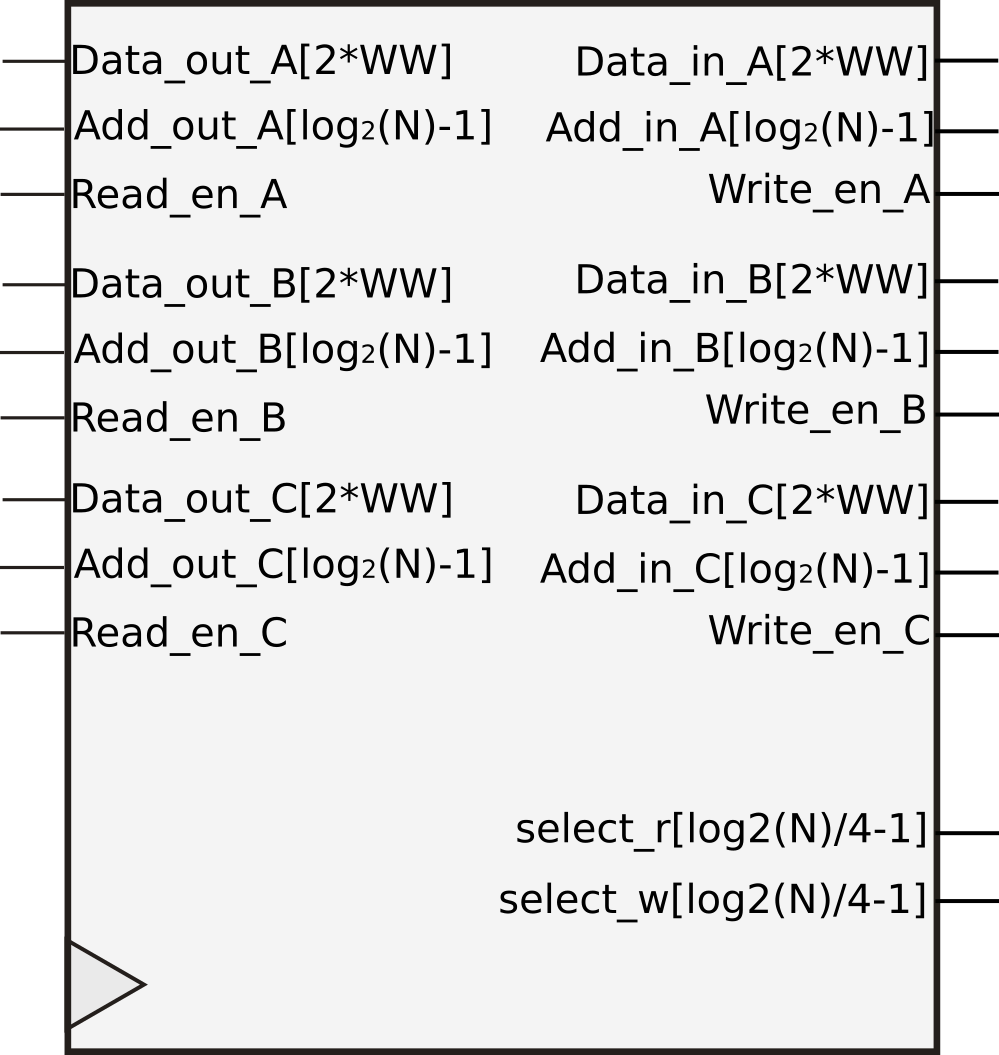
\includegraphics[width=6cm]{./figures/tripleRAM.png}
        \caption{RAM de triple entrada y triple salida}
        \label{fig:tripleRam}
\end{figure}

El bloque tiene tres puertos de entrada y tres puertos de
salida, cada uno con sus correspondientes señales de datos, dirección y habilitación. Las señales
select\_r y select\_w se utilizan para determinar, en conjunto con la señal de dirección de cada
puerto, en que región de la memoria esribir.\\

Como es necesario poder leer y escribir en tres posiciones de memoria simultáneas se construye el
bloque de memoria RAM de triple entrada y triple salida utilizando tres subbloques RAM de doble
puerto igual a los utilizados en la radix-2 (subsección \ref{sec:r2mem}). Se hace de esta manera ya que al
sintetizar en una FPGA, los bloques de memoria RAM de doble puerto se sintetizan utilizando los
bloques RAM propios de la FPGA optimizando la utilización de recursos.


Cada uno de los tres subbloques RAM que componen el bloque triple tiene una capacidad de
almacenamiento de $N/3$ puntos. La distribución de los puntos en los tres subbloques se realiaza de
forma que en cada operación aritmética de cuatro puntos, haya un punto entrando a la unidad
aritmética desde la entrada a la arquitectura o desde la etapa anterior y los restantes tres
provenientes de cada uno de los subbloques RAM, para obtenerlos en forma simultánea. Del mismo
modo, de los cuatro resultados de la operación aritmética, uno se reserva para la etapa siguiente y
los tres restantes se almacenan cada uno en sendos subbloques RAM simultáneamente.

Como el acceso a las posiciones de memoria no es siempre a direcciones continuas, ya que al ser una
arquitectura iterativa se ejecuta sucesivamente una operación de cada etapa, se direccionan los
subbloques de memoria de manera que queden delimitadas las porciones de memoria correspondientes a
cada etapa, como se muestra en la figura \ref{fig:tripleRamdir}. Cada una de estas regiones es de
tamaño igual a $\frac{1}{4}$ de la longitud de la FFT de la etapa correspondiente, por ejemplo la porción de memoria correspondiente a la primer etapa
será $\frac{N}{4}$ en cada subbloque, comprendiendo en total $\frac{3N}{4}$, para la segunda
etapa cada subbloque reservará $\frac{\log_4(N)}{4}$ ya que cada FFT de la segunda etapa es de
longitud $\log_4(N)$, así hasta llegar a la última etapa donde solo se reserva una posición de
memoria de cada subbloque, almacenando en el bloque completo los tres puntos necesarios para
realizar un cálculo aritmético cuando llegue el siguiente punto de la etapa
anterior.

Para direccionar la memoria se utiliza un vector de dirección de $\log_2(N)-1$, que si bien
permitiría direccionar $N/2$ posiciones de memoria aquí se lo utiliza para direccionar $N/3$ ya que
un vector de direcciones de $\log_2(N)-2$ solo permite direccionar $N/4$ posiciones.
Para obtener la dirección de la posición que se debe leer o escribir se utiliza como base el
contenido de la entrada de dirección del subbloque correpondiente y se le aplica un enmascarado con
el valor de la entrada de selección (select\_r o select\_w) que asignan valores a los bits de mayor
valor de la palabra de dirección, permitiendo así leer o escribir en la posición respectiva a la
dirección base en la región que corresponda a la etapa actual del cómputo de la FFT.

\begin{figure}[htb!]
        \centering
        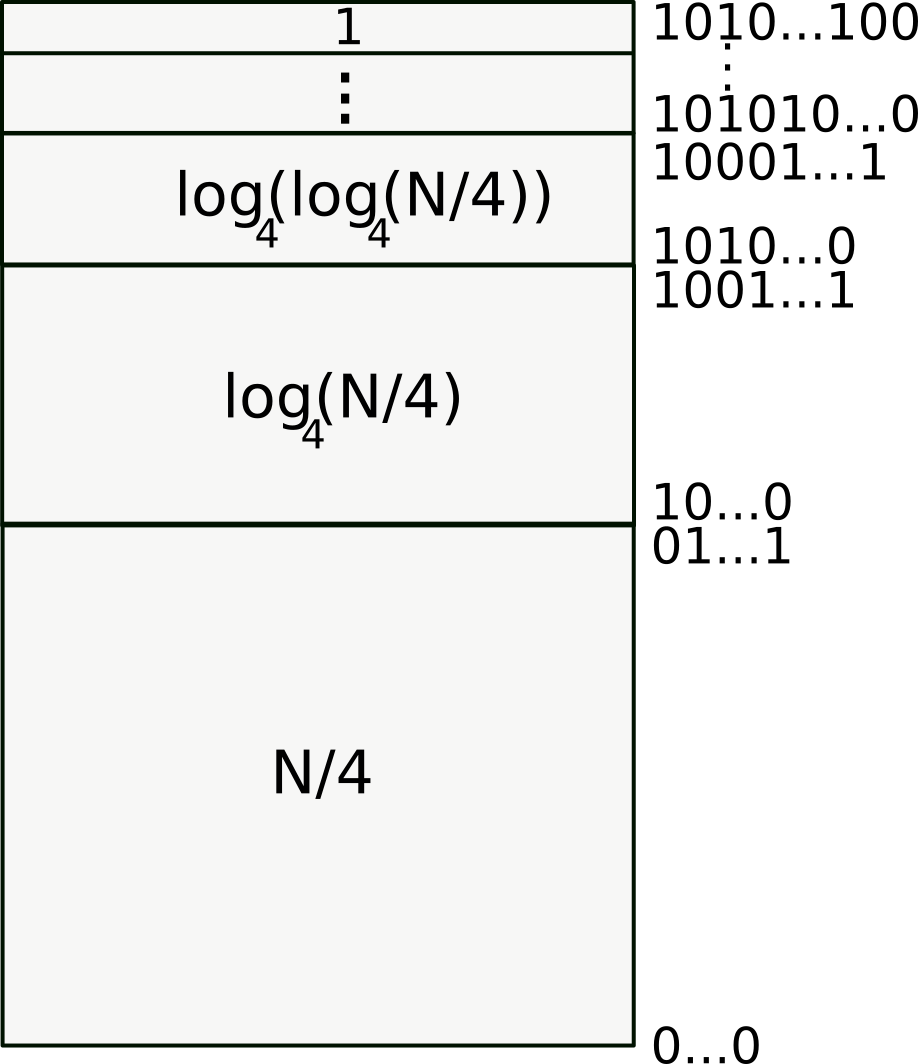
\includegraphics[width=6cm]{./figures/tripleRAMdir.png}
        \caption{Esquema de direccionamiento de los subbloques RAM}
        \label{fig:tripleRamdir}
\end{figure}

En la figura \ref{fig:tripleRamdir} se muestra esquemáticamente la división de cada subbloque en
regiones a través del direccionado, y las direcciones respectivas al comienzo y final de cada
región. Se ve claramente como quedan direcciones sin utilizar ya que con $\log_2(N)-1$ bits se
podrían direccionar $N/2$ posiciones de memoria, por lo que se utilizan únicamente $2/3$ de las
direcciones posibles.

A través de los controles de habilitación de lectura y escritura se puede acceder individualmente a
cada subbloque RAM de la memoria de triple entrada y triple salida.

\subsection{Sumador/restador}

La unidad aritmética debe resolver las ecuaciones (\ref{eq:radix4_suby}) a (\ref{eq:radix4_subh}).
Para esto se opera directamente transladando dichas ecuaciones a \textit{verilog} teniendo en cuenta
que multiplicar por $j$ es equivalente a intercambiar las partes real e imaginaria (canbiando el
signo de la última) del número complejo. Por la forma que toma cada operación de cuatro puntos en el
diagrama de la figura \ref{fig:r4_diag} se le llama \textit{dragonfly} a la unidad de cómputo
aritmético de la radix-4.

En cada etapa del cómputo de la radix-4 pueden realizarse dos tipos de operaciones, una operación
aritmética entre cuatro puntos o un movimiento de datos en memoria, como sucede en la radix-2. En el
segundo caso, el movimiento a memoria puede ser el almacenamiento de un punto entrante a la arquitectura o
proveniente de una etapa anterior, o la lectura de un punto de memoria para multiplicarlo por un
twiddle factor y almacenarlo nuevamente en la región correspondiente a la etapa siguiente
(corresponde al traspaso de un punto resultante de una operación aritmética de una etapa a la
siguiente pasando por el multiplicador). 
Para las operaciones de movimientos de datos en memoria se
dispone internamente en la unidad aritmética de un sistema de multiplexores que permiten direccionar
la entrada del dato de la arquitectura a cualquiera de las tres salidas correspondientes a los tres
subbloques de memoria para su almacenamiento, o direccionar cualquiera de las tres entradas desde
memoria a la salida conectada a la entrada del multiplicador para realizar el traspaso de puntos de
una etapa a la siguiente.

\begin{figure}[htb!]
        \centering
        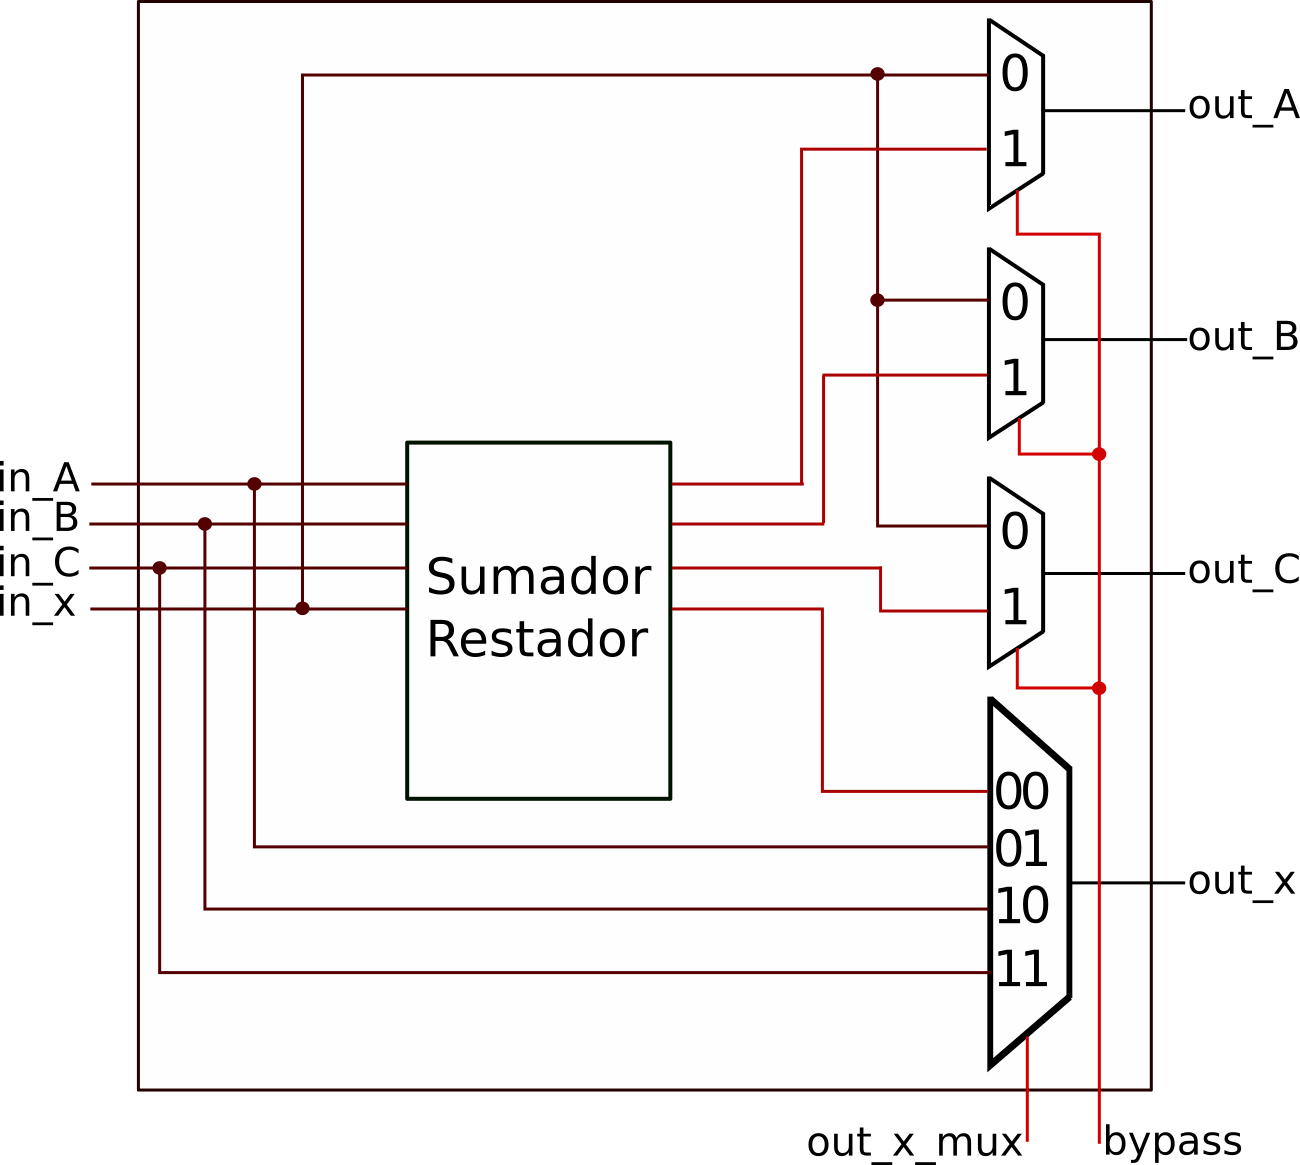
\includegraphics[width=8cm]{./figures/firefly.png}
        \caption{Diagrama de la unidad aritmética incluyendo los multiplexores de bypass}
        \label{fig:firefly}
\end{figure}

En la figura \ref{fig:firefly} se muestra el diagrama en bloque de la unidad aritmética. Se observa
el arreglo de multiplexores que permite direccionar a las salidas a memoria los resultados de la
operación aritmética o la entrada $x$ del bloque. También se observa un multiplexor $4-1$ que
permite seleccionar la salida $x$, conectada al multiplicador, que permite seleccionar entre el
resultado de la operación aritmética o una de las tres entradas de operandos $A, B$ o $C$. 
La unidad aritmética incluye los mecanismos para realizar el redondeo o truncamiento, controlados
por dos señales: una señal de selección de redondeo o truncamiento y una señal de habilitación de 
redondeo/truncamiento individual por etapa. Este mecanismo se detalla en la subsección
\ref{sec:secEscal}.\\
Para almacenar en memoria un dato entrante a la arquitectura se direcciona al subbloque de memoria
correspondiente a través del módulo \textit{dragonfly}, al igual que al extraer un dato de un
subbloque de memoria para enviarlo a la salida de la arquitectura.

\subsection{Datapath}
En la figura \ref{fig:datapathR4} se observa el datapath para la radix-4 iterativa. El bloque
\textit{dragonfly} concentra la unidad aritmética, el algoritmo de redondeo/truncado y el datapath
interno que distribuye las entradas en las diferentes salidas. Los datos entrantes a cada subbloque
de memoria pueden provenir desde la unidad aritmética como resultado de una operación o desde el
\textit{delay register}, proveniente de la etapa anterior.

\begin{figure}[htb!]
        \centering
        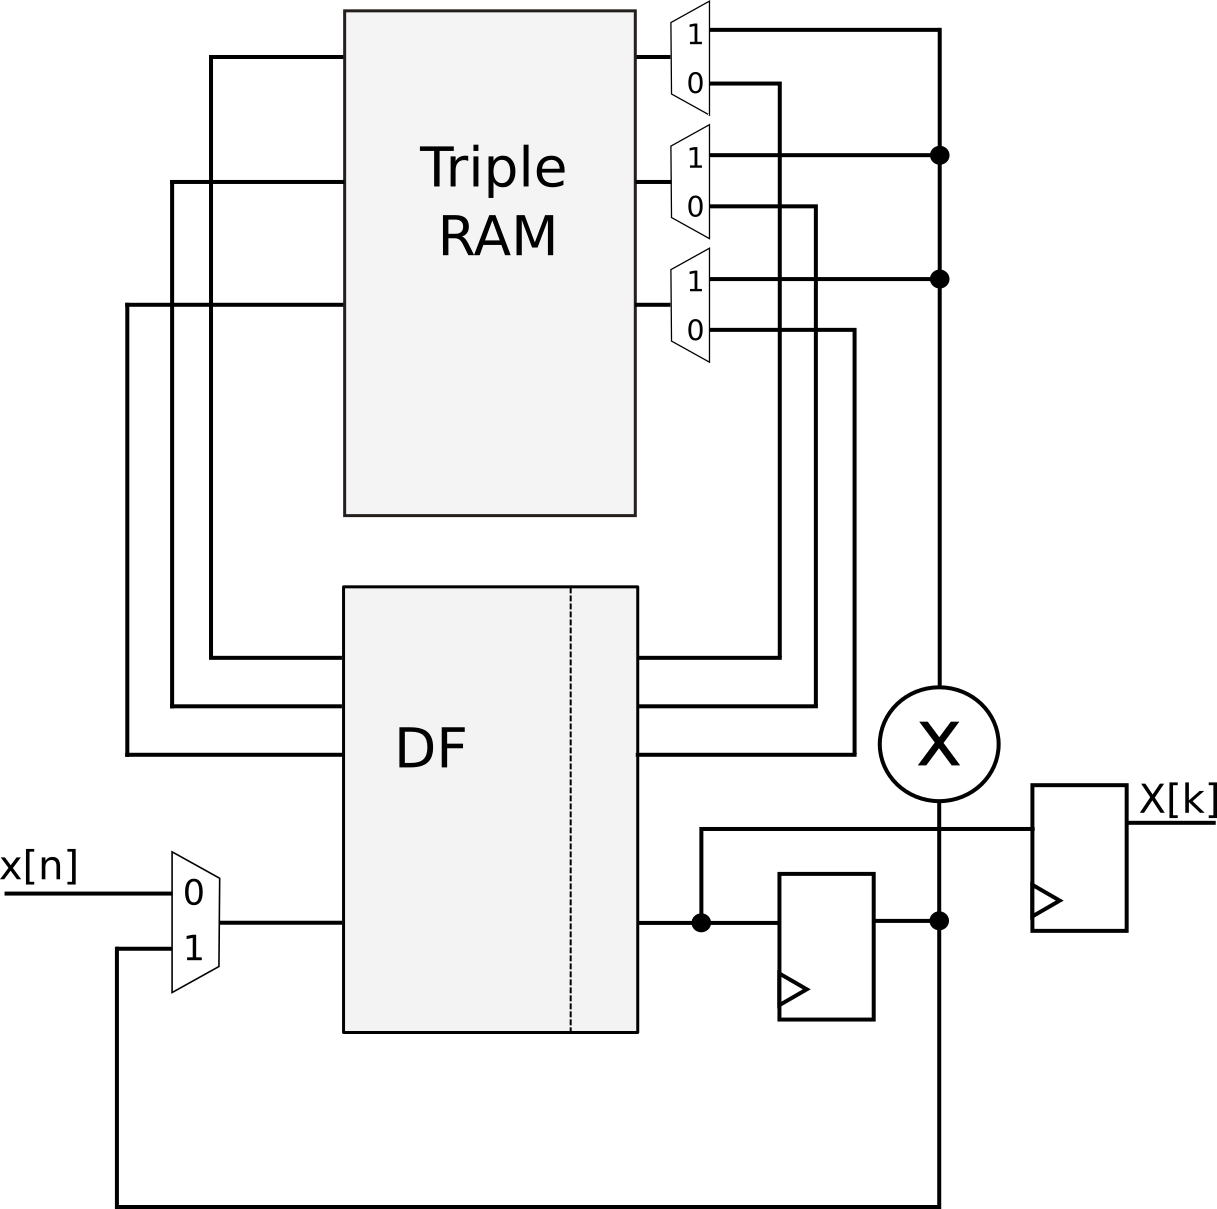
\includegraphics[width=8cm]{./figures/datapathR4.png}
        \caption{Datapath de la arquitectura radix-4 iterativa}
        \label{fig:datapathR4}
\end{figure}

El \textit{datapath} es controlado por la unidad de control a través de los multiplexores de acceso
a memoria, el mumltiplexor de entrada a la unidad aritmética y el \textit{datapath} interno de la
unidad aritmética por medio de sus señales de control.

En la figura \ref{fig:datapathMemR4} se muestran las posibles configuraciones para el
\textit{datapath} para operaciones de transferencia a memoria de acuerdo al tipo de etapa que se
está procesando.
Las líneas punteadas muestran caminos posibles dependiendo del subbloque de memoria donde se desea escribir o leer.

Durante estas operaciones, dependiendo de si la entrada es inicial, intermedia o final, se toma el
dato de entrada de la arquitectura o de la etapa anterior y se envía a memoria, y se lee un dato de
memoria y se envía al \textit{delay register} para ser luego multiplicado por el twiddle factor y
ser guardado en memoria en la etapa siguiente, o enviado a la salida de la arquitectura en caso
de estar ejecutándose la etapa final.\\

\begin{figure}[htb!]
        \centering
        \begin{subfigure}{\columnwidth}\centering
        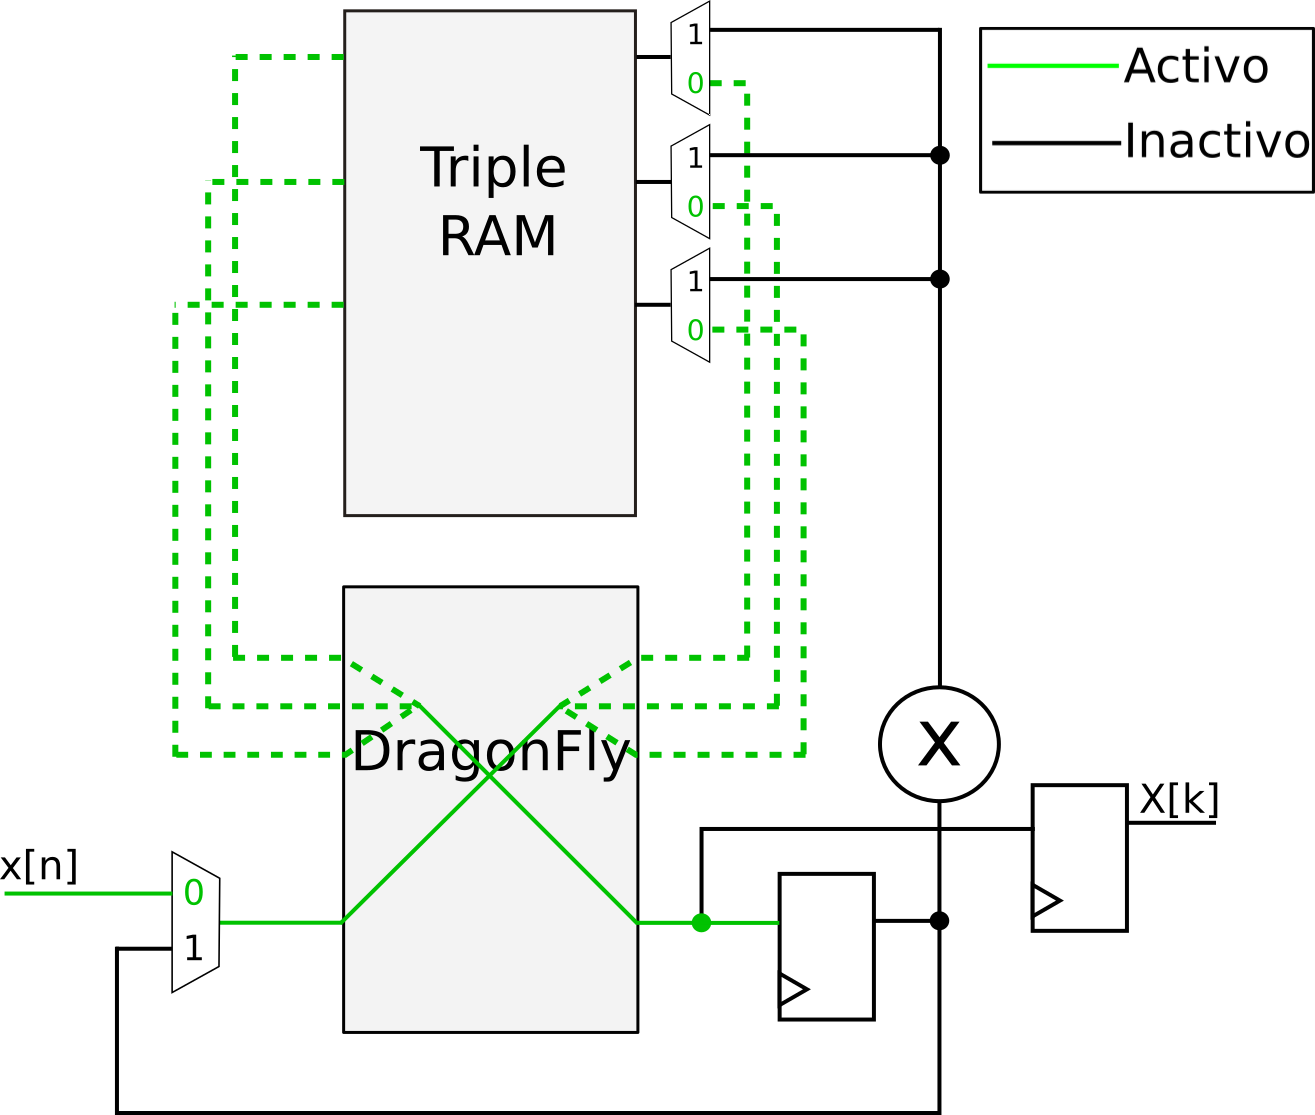
\includegraphics[width=7cm]{./figures/datapathR4_mem_ini.png}
        \caption{Etapa inicial}
        \end{subfigure}
        \begin{subfigure}{\columnwidth}\centering
        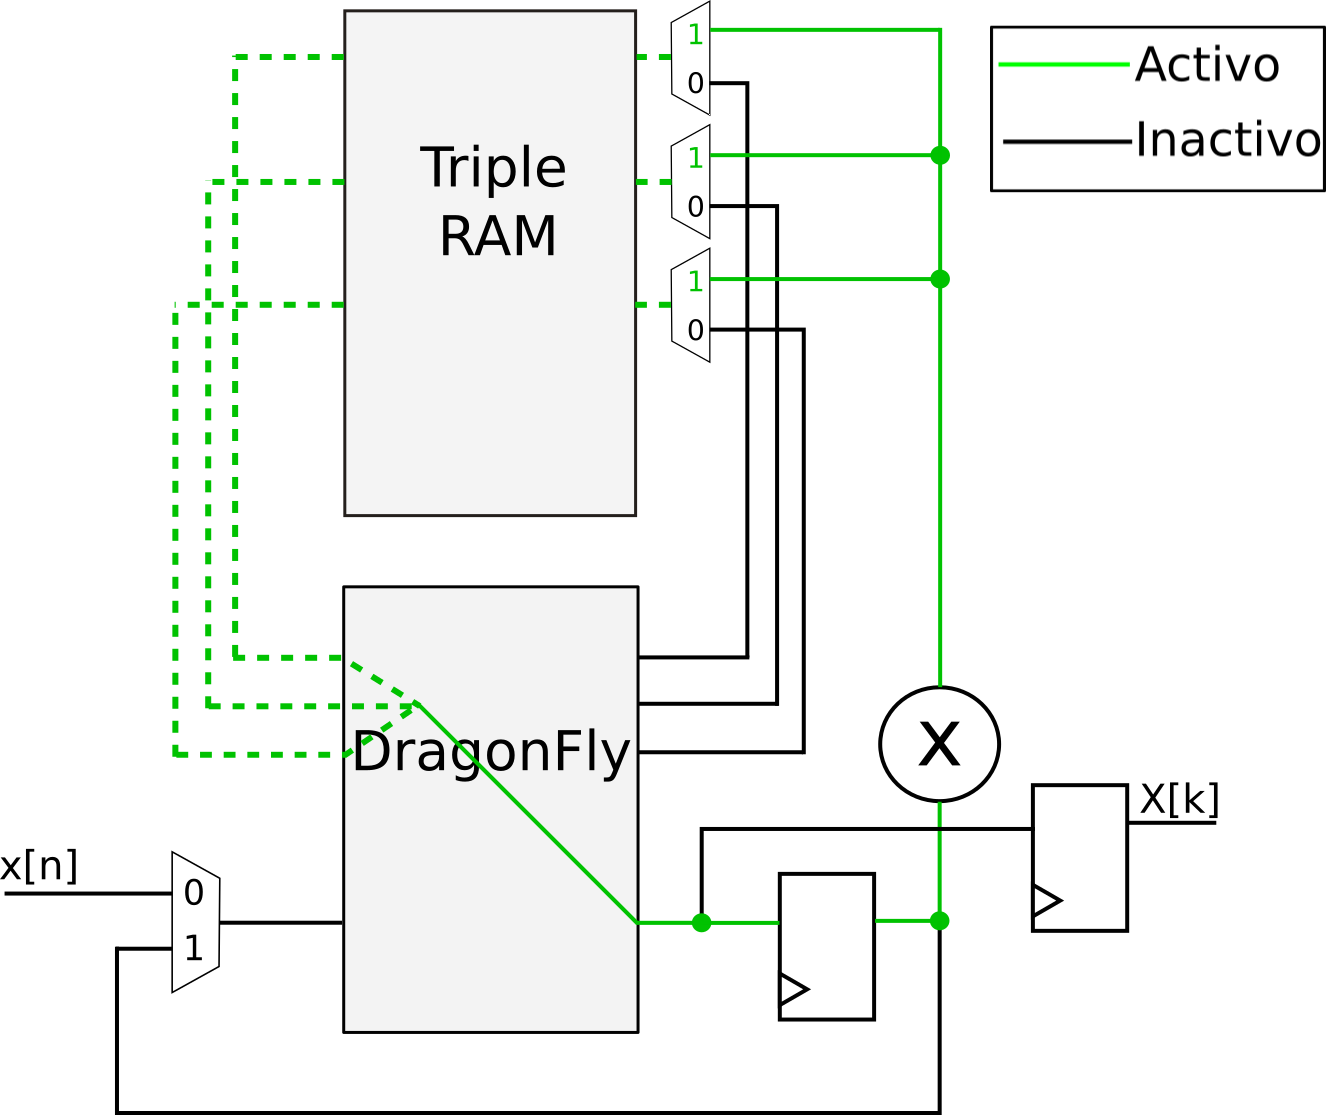
\includegraphics[width=7cm]{./figures/datapathR4_mem_int.png}
        \caption{Etapa intermedia}
        \end{subfigure}
        \begin{subfigure}{\columnwidth}\centering
        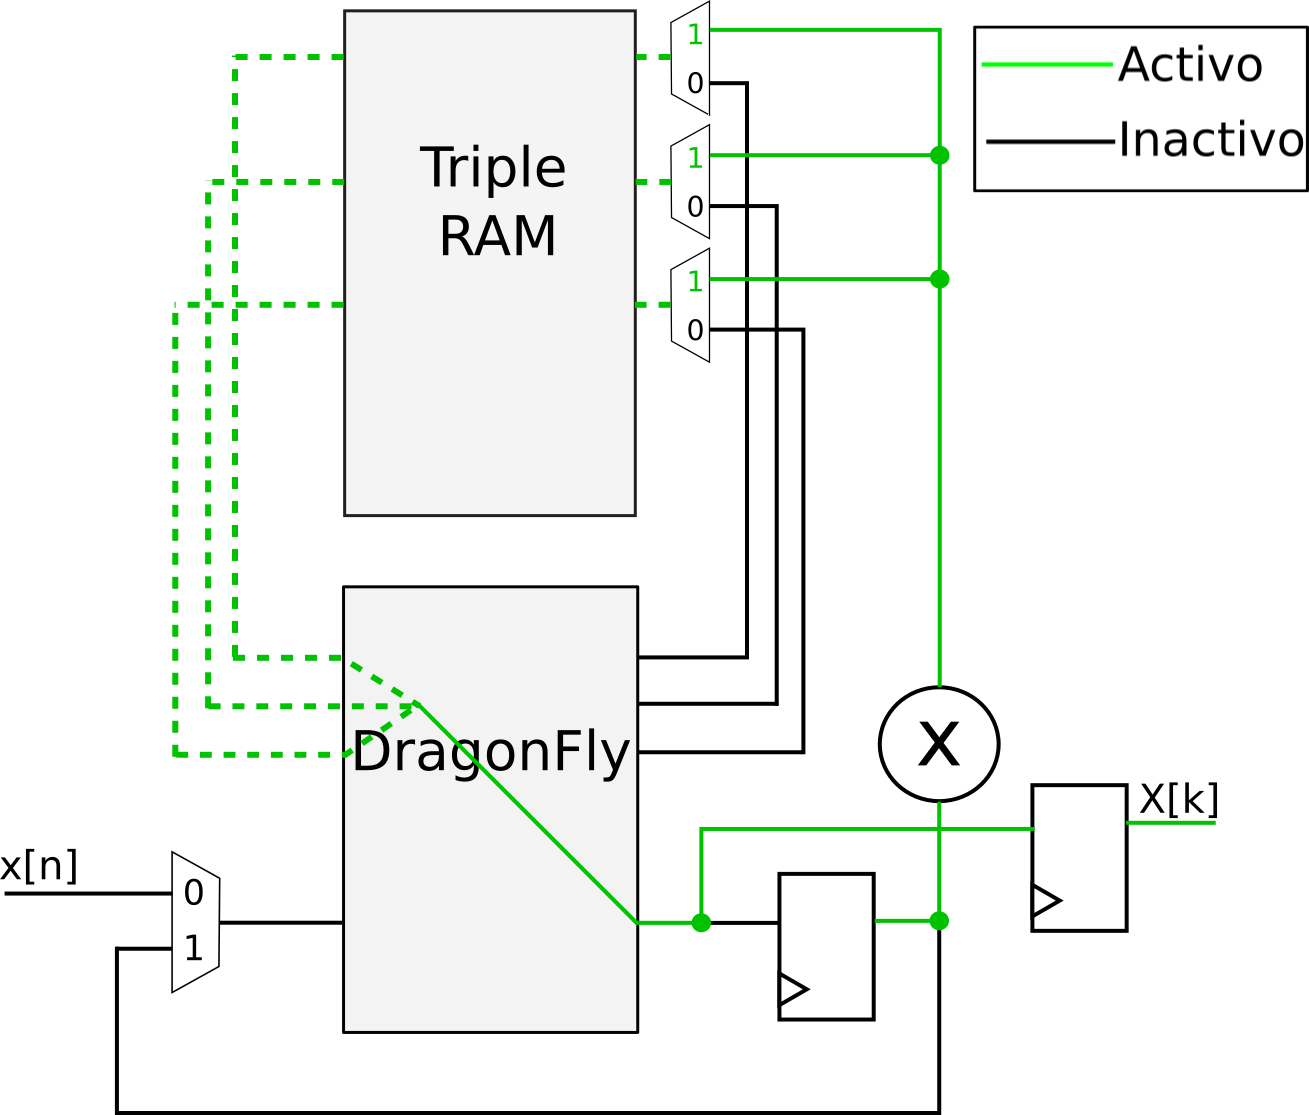
\includegraphics[width=7cm]{./figures/datapathR4_mem_fin.png}
        \caption{Etapa final}
        \end{subfigure}
        \caption{Datapath para operaciones de transferencia en memoria}
        \label{fig:datapathMemR4}
\end{figure}

En la figura \ref{fig:datapathAritR4} se muestran las distintas configuraciones posibles para el
\textit{datapath} para operaciones aritméticas.

Durante estas operaciones se leen tres datos almacenados en memoria y un dato, que dependiendo de si
la etapa que se está procesando es la inicial, una etapa intermedia o la etapa final, proviene de la
entrada de la arquitectura o de la etapa anterior y se los procesa en la unidad aritmética. Una vez
realizada la operación, tres de los resultados son almacenados en memoria y el restante se envía al
\textit{delay register} para su utilización en la etapa siguiente, en caso de estar procesando la
etapa inicial o una etapa intermedia, o a la salida de la arquitectura en caso de ser la etapa
final.

\begin{figure}[htb!]
        \centering
        \begin{subfigure}{\columnwidth}\centering
        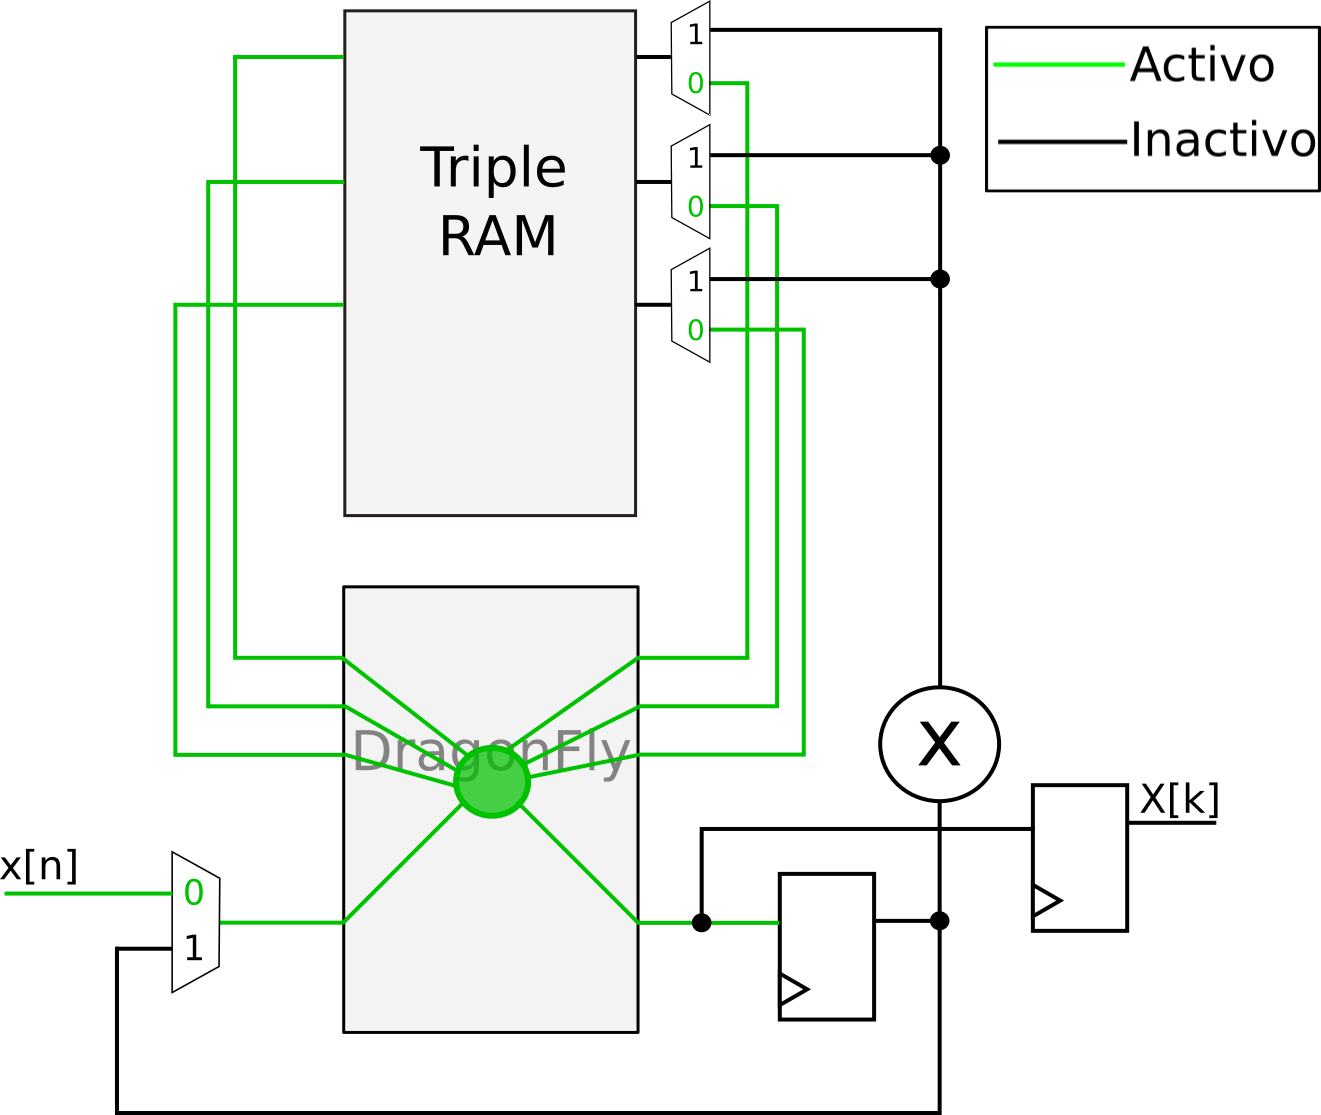
\includegraphics[width=7cm]{./figures/datapathR4_arit_ini.png}
        \caption{Etapa inicial}
        \end{subfigure}
        \begin{subfigure}{\columnwidth}\centering
        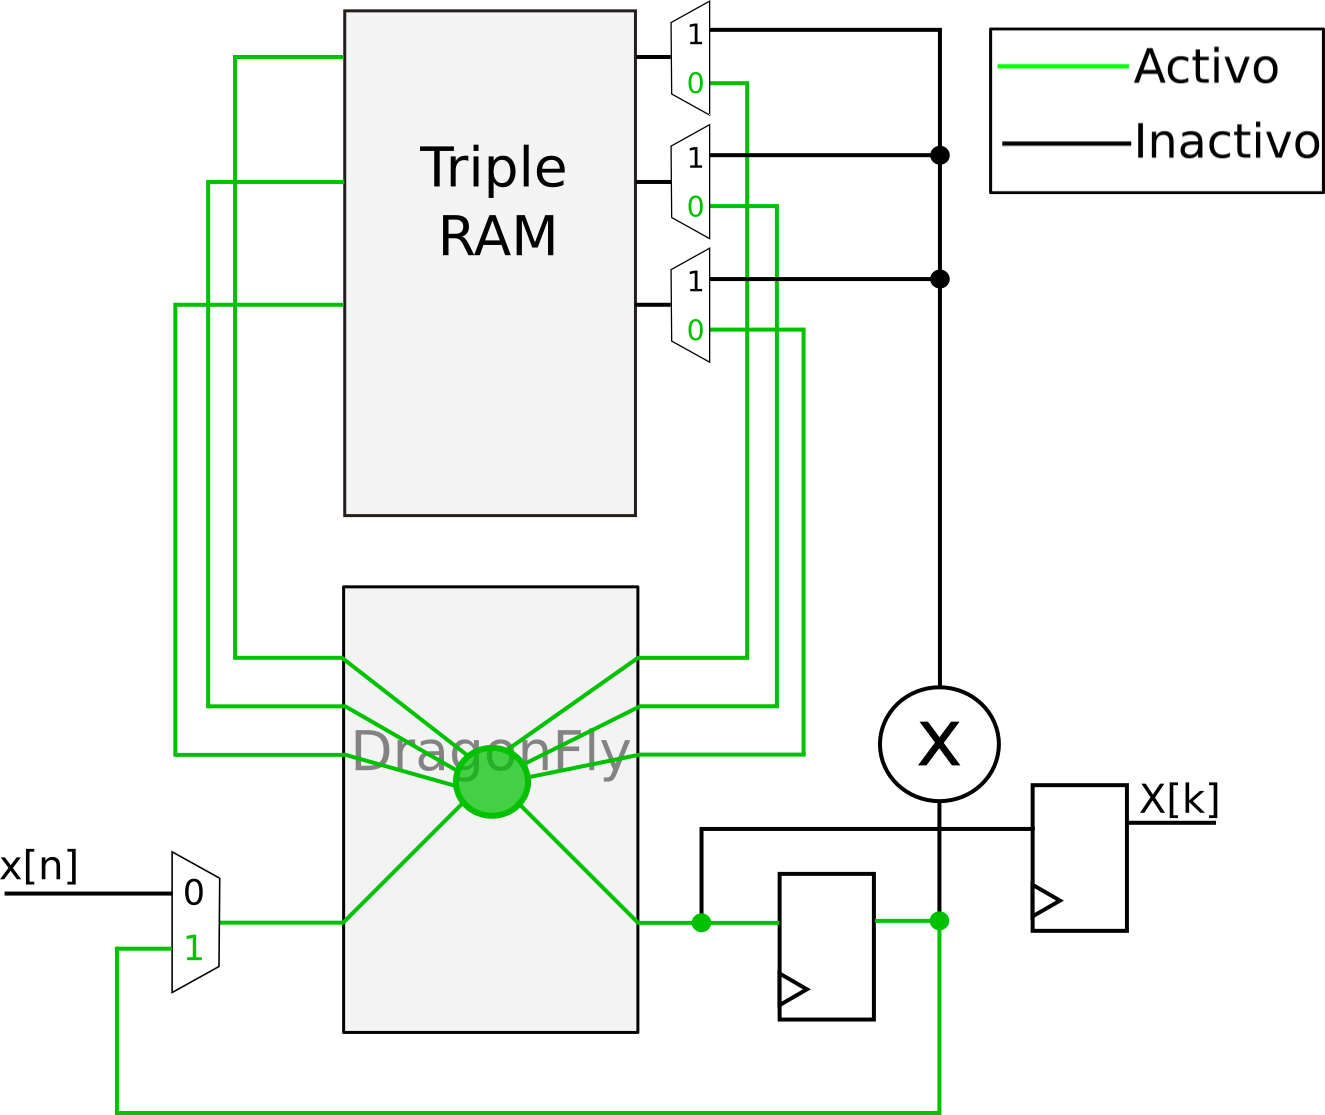
\includegraphics[width=7cm]{./figures/datapathR4_arit_int.png}
        \caption{Etapa intermedia}
        \end{subfigure}
        \begin{subfigure}{\columnwidth}\centering
        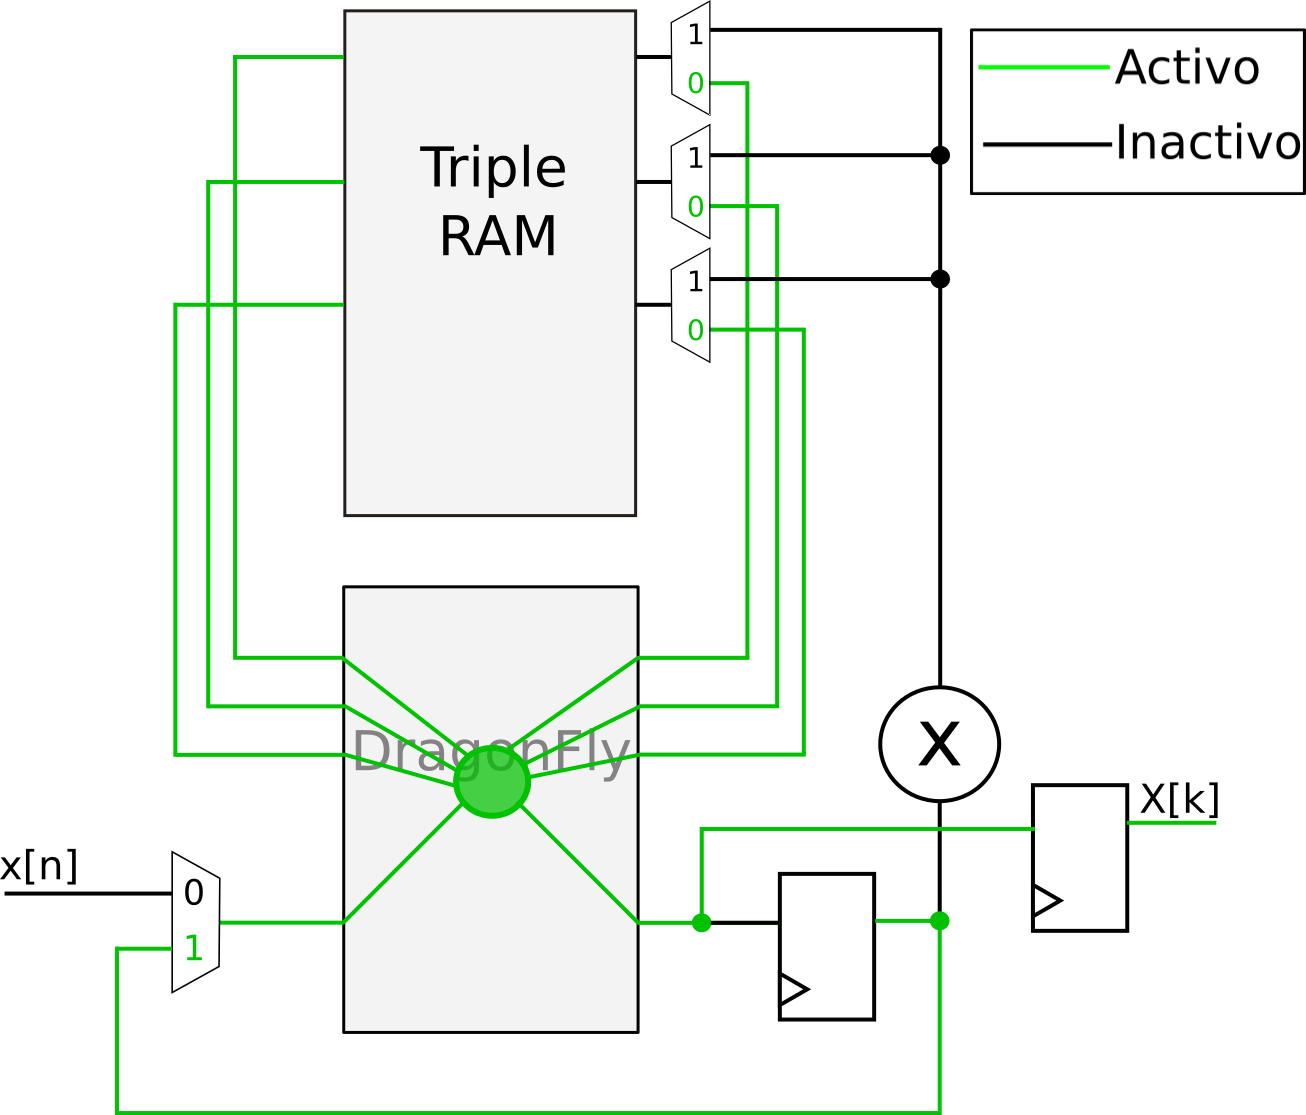
\includegraphics[width=7cm]{./figures/datapathR4_arit_fin.png}
        \caption{Etapa final}
        \end{subfigure}
        \caption{Datapath para operaciones en butterfly}
        \label{fig:datapathAritR4}
\end{figure}

En la arquitectura radix-4 iterativa propuesta se pueden identificar tres tipos distintos de etapas,
la etapa inicial, las intermedias y la final, en las que pueden ejecutarse una de dos posibles
operaciones: una transferencia de un dato a memoria o una operación aritmética. El tipo de etapa
que se está procesando y el tipo de operación que se realiza en esa etapa determinan la
configuración del datapath en cada ciclo de \textit{clock}.\\

A continuación se listan las posibles configuraciones de \textit{datapath} para cada tipo de etapa y
operación:

\begin{itemize}
  \item Etapa inicial
  \begin{itemize}
    \item Operaciones aritméticas: tres datos almacenados en memoria y el dato
    de entrada a la arquitectura. Tres de los resultados son almacenados en memoria mientras que el
    cuarto se envía al multiplicador.
    \item Transferencia a memoria: se almacena el dato entrante a la arquitectura en uno de los tres
    subbloques de memoria.
  \end{itemize}
  \item Etapas intermedias
  \begin{itemize}
    \item Operaciones aritméticas: tres datos almacenados en memoria y el dato de la etapa anterior
    alacenado en el \textit{delay register}. Tres de los resultados son almacenados en memoria mientras que el
    cuarto se envía al multiplicador.
    \item Transferencia a memoria: se extrae un dato de memoria y se envía al multiplicador mientras
    se almacena en memoria el dato de la etapa anterior almacenado en el \textit{delay register}.
  \end{itemize}
  \item Etapa final
  \begin{itemize}
    \item Operaciones aritméticas: tres datos almacenados en memoria y el dato de la etapa anterior
    alacenado en el \textit{delay register}. Tres de los resultados son almacenados en memoria mientras que el
    cuarto se envía a la salida de la arquitectura.
    \item Transferencia a memoria: se extrae un dato de memoria y se envía a la salida de la
    arquitectura mientras se almacena en memoria el dato de la etapa anterior almacenado en el
    \textit{delay register}.
  \end{itemize}
\end{itemize}

\subsection{Unidad de control}

La unidad de control debe contener la lógica necesaria para controlar el funcionamiento de la
arquitectura. Está compuesta por una máquina de estados principal que controla el funcionamiento
general de la arquitectura, y una máquina de estados secundaria que configura el \textit{datapath}
de acuerdo al tipo de etapa y operación que se debe procesar.\\
La unidad de control además de configurar el \textit{datapath} debe controlar el direccionamiento de
la memoria, así como sus señales de control, y generar los \textit{twiddle factors} para el
multiplicador.\\

Al tratarse de una arquitectura radix-4, entra a la arquitectura un punto cada $\log_4(N)$ ciclos de
\textit{clock}, y este es también el número de etapas de la arquitectura, se tiene  un contador de
longitud $\log_2(\log_4(N))$ puntos para identificar el estado que se está procesando en cada ciclo
de \textit{clock}. El desborde de este contador alimenta un contador de longitud $\log_2(N)$ que
cuenta la cantidad de puntos que han ingresado a la arquitectura y permite controlar en que estado
del cómputo total se encuentra. Con estos dos contadores se lleva el control de la máquina de
estados que controla el \textit{datapath} y la memoria, y la generación de los \textit{twiddle
factors}.

Como se ve en la figura \ref{fig:r4_diag}, para una radix-4 de $16$ puntos, en la primer etapa hay
que almacenar en memoria los primeros $12$ puntos hasta realizar una operación aritmética con el
decimotercer punto que entra, utilizando también el primer punto, el quinto y el noveno. En la
segunda etapa se deben almcenar los primeros tres puntos que llegan y recién realizar la operación 
aritmética con el cuarto punto. Cada almacenamiento en memoria puede hacerse a uno de los tres
subbloques, por lo que debe diferenciarse a que subbloque pertenece cada punto que ingresa a una
etapa.

Para decidir si se debe realizar una operación aritmética o una transferencia a memoria, y en este
caso en que se subbloque se debe almacenar el dato, se utilizan dos bits del contador de puntos de
la siguiente manera:

\begin{itemize}
  \item $[00]$ ->  Almacenamiento en subbloque de memoria 1
  \item $[01]$ ->  Almacenamiento en subbloque de memoria 2
  \item $[10]$ ->  Almacenamiento en subbloque de memoria 3
  \item $[11]$ ->  Operación aritmética 
\end{itemize}

Los dos bits del contador de puntos utilizados para determinar la operación a realizar dependen de
la etapa, por lo que se seleccionan de acuerdo al \textit{stg\_ctr} como se muestra en la
\ref{fig:r4conts} para una arquitectura radix-4 de 256 puntos.
 
% Como se explicó en la sección \ref{sec:r4mem}, los subbloques deben almacenar los puntos de manera
% que en cada operación aritmética se encuentre cada uno de los tres datos a extraer de memoria en
% subloques diferentes. Por esto, para la primer etapa del diagrama de la figura \ref{fig:r4_diag} se
% deben almacenar en cada subbloque cuatro puntos en forma consecutiva y luego pasar al subbloque
% siguiente. Para lograr esta diferenciación se leen los bits del contador de puntos de a pares
% utilizando el contador de etapas como índice, comenzando del bit más alto del contador de puntos,
% como se indica en la figura \ref{fig:r4conts}, ejemplificando con dos pares de bits para valores del
% contador de estados (\textit{st\_ctr}) de $0$ y $2$.

\begin{figure}[htb!]
        \centering
        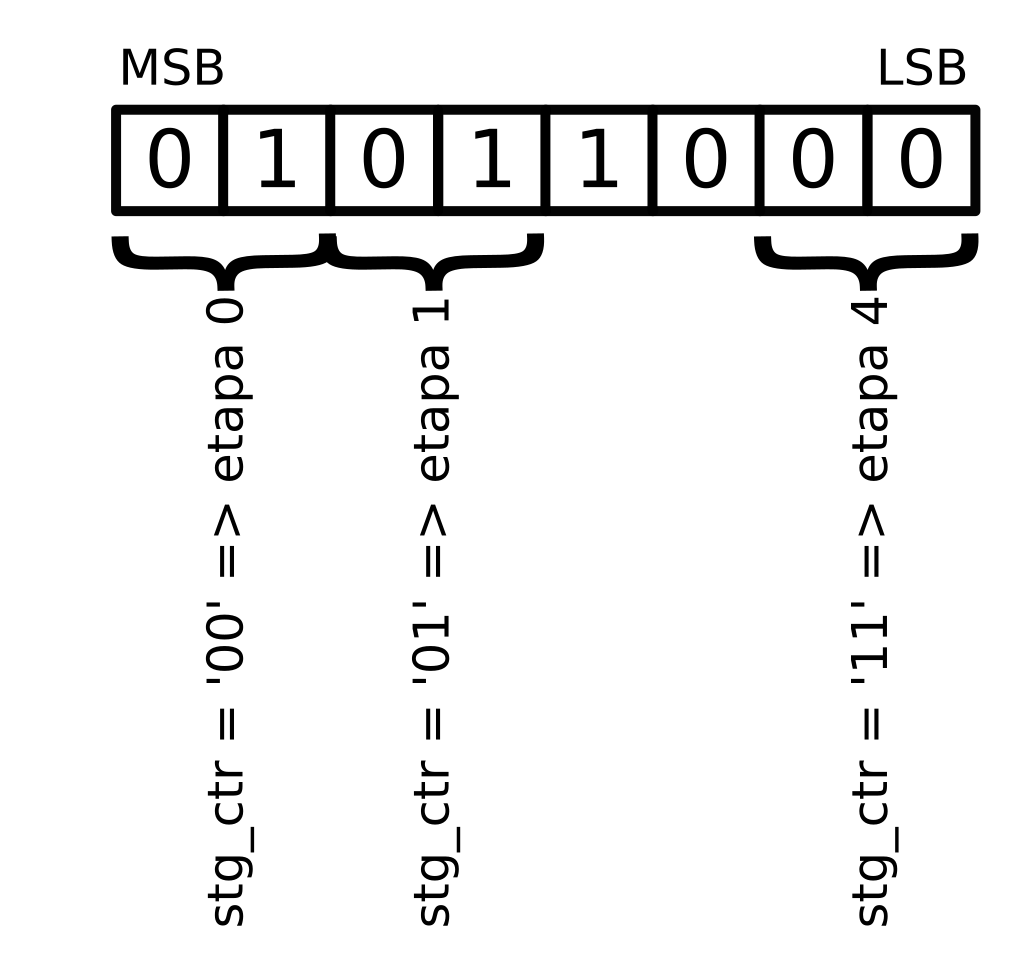
\includegraphics[width=6cm]{./figures/r4conts.png}
        \caption{Selección del par de bits del contador de puntos a evaluar}
        \label{fig:r4conts}
\end{figure}

\subsubsection{Máquinas de estados}

En la figura \ref{fig:r4statep} se muestra el diagrama de estados y transiciones la máquina de
estados principal.
El estado
\textit{Idle} es el estado inicial de la arquitectura. La señal start pasa la máquina al estado \textit{Init}
donde inicializa los parámetros de la arquitectura necesarios para comenzar a procesar y lee el
primer dato de entrada a la arquitectura. Un ciclo de \textit{clock} después la máquina pasa
automáticamente al estado \textit{enabled}.

\begin{figure}[htb!]
        \centering
        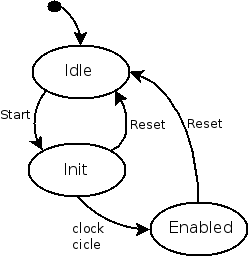
\includegraphics[width=7cm]{./figures/SMr2gen.png}
        \caption{Diagrama de estados y transiciones de la máquina de estados principal}
        \label{fig:r4statep}
\end{figure}

En el estado \textit{Enabled} se identifica la etapa que se está procesando y se configura el
\textit{datapath} para realizar la operación correspondiente. Para esto se utiliza la máquina de
estados secundaria, cuyo estado depende del valor de los bits del contador de puntos
correspondientes a la etapa actual.

\begin{figure}[htb!]
        \centering
        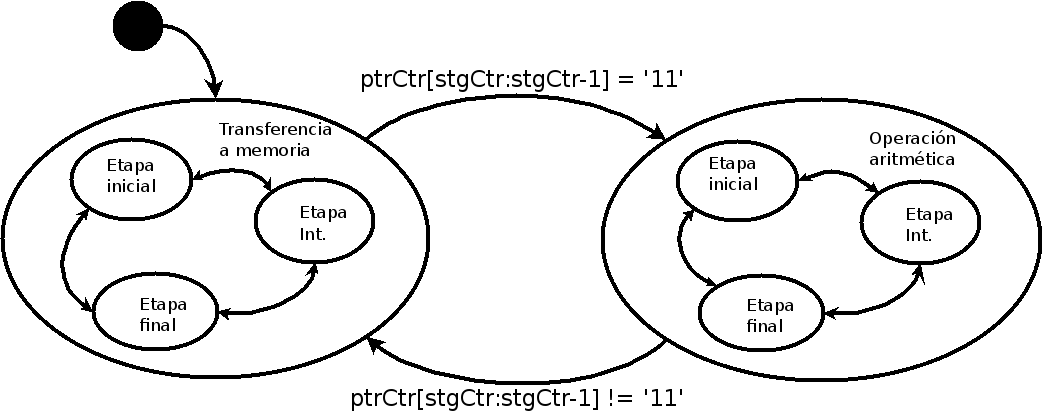
\includegraphics[width=13cm]{./figures/SMr4op.png}
        \caption{Diagrama de estados y transiciones de la máquina de estados secundaria}
        \label{fig:r4stateop}
\end{figure}

En la figura \ref{fig:r4stateop} se observa la máquina de estados secundaria. Dentro de cada uno de
los estados principales se evalúa el tipo de etapa para la configuración del \textit{datapath}.
En cada uno de los estados principales funciona una submáquina de estados que realiza ajustes
menores de acuerdo a si la etapa actual es la etapa inicial, una intermedia o la etapa final. $ptrCtr[stgCtr:stgCtr-1]$ hace
referencia a los dos bits del contador de puntos correspondientes al valor del contador de etapas.\\
Esta máquina de estados controla además la señal de habilitación de escalamiento para la etapa
actual de acuerdo al vector de escalamiento de entrada a la arquitectura. También controla, a través
del contador de puntos y el de etapas, las señales de \textit{handshaking} de salida, indicando si
el dato de salida es un dato válido, señal \textit{data\_valid} y si es el punto inicial o final de
la FFT que se está procesanto actualmente, señales \textit{soo} y \textit{done} respectivamente.

\subsubsection{Control de la memoria}

El control de la memoria se realiza mediante los direccionamientos, las señales de habilitación de
lectura y escritura, y las señales de selección de la región de memoria de cada subbloque donde se
realizará la operación.

El direccionamiento de escritura se realiza directamente mapeando el valor del contador de puntos a
la dirección de escritura. El direccionamiento de lectura se realiza mapeando a la dirección de
lectura el valor del contador de puntos correspondiente al ciclo siguiente de \textit{clock} ya que
en cada flanco positivo del \textit{clock} la memoria dispone a la salida el dato guardado en la
dirección presente en el puerto de dirección de lectura durante el flanco.

Las señales de habilitación de lectura y escritura se controlan dependiendo del valor de los bits
correspondientes del contador de puntos, habilitando el subbloque de memoria correspondiente para
los casos de movimientos en memoria y habilitando los tres subbloques simultáneamente para el caso
de operaciones aritméticas.

Las señales de selección de la región de memoria se controlan utilizando el contador de etapas, ya
que cada región de memoria en un subbloque particular se utiliza para una etapa determinada. Las
señales de selección se construyen como una máscara para lo bits superiores de la señal de
direccionamiento, para ubicar la dirección indicada por el contador de puntos en la región
correspondiente.

\subsection{Integración de la unidad de control}

En la figura \ref{fig:datapathR4control} se muestra el diagrama del \textit{datapath} de la figura
\ref{fig:datapathR4} con el agregado de las señales de la unidad de control. 

\begin{figure}[htb!]
        \centering
        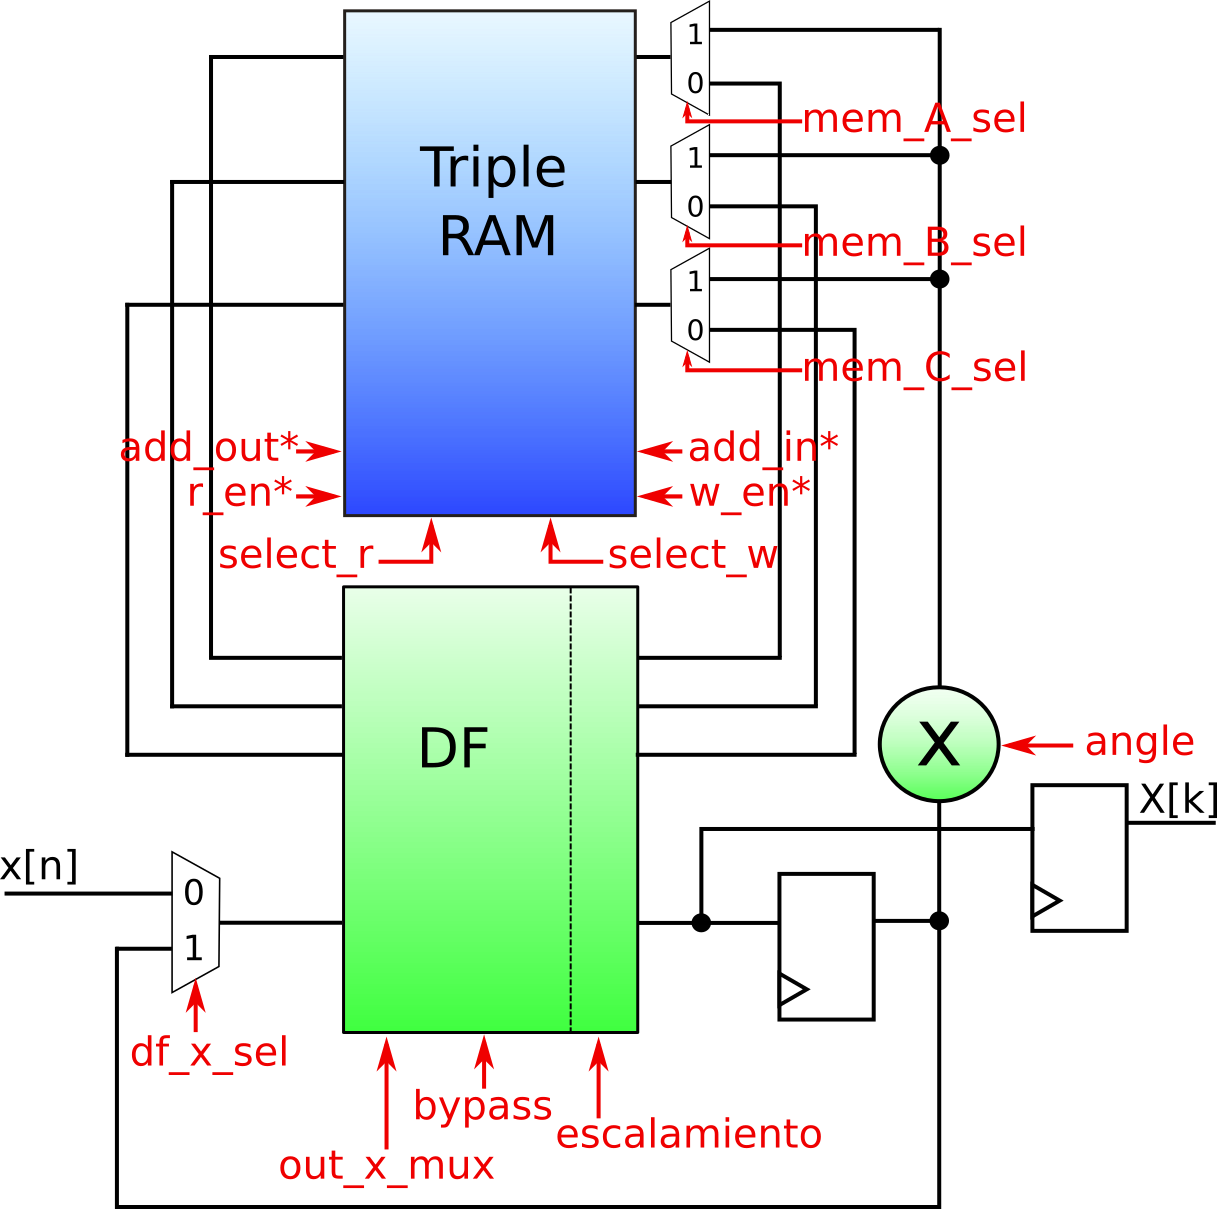
\includegraphics[width=9cm]{./figures/datapathR4control.png}
        \caption{Datapath con las señales de control}
        \label{fig:datapathR4control}
\end{figure}

Las señales de control de la figura \ref{fig:datapathR4control} se listan a continuación, indicando
entre parétesis su tamaño si es mayor a $1$:

\begin{itemize}
  \item \textbf{add\_in*} ($\log_2(N)$) \textit{address in}, dirección de memoria donde se escribirá
  el dato.
  \item \textbf{w\_en*} \textit{write enable}, señal de habilitación de escritura en memoria
  \item \textbf{add\_out*} ($\log_2(N)$) \textit{address out}, dirección de memoria a la que se
  desea acceder.
  \item \textbf{r\_en*} \textit{read enable}, señal de habilitacón de lectura de memoria
  \item \textbf{select\_r} ($\log_2(\log_4(N)))$) Selección de la región de memoria donde se realiza
  la lectura.
  \item \textbf{select\_r} ($\log_2(\log_4(N)))$) Selección de la región de memoria donde se realiza
  la escritura.
  \item \textbf{mem\_A\_sel} señal de control del multiplexor a la entrada al subbloque A de la
  memoria.
  \item \textbf{mem\_B\_sel} señal de control del multiplexor a la entrada al subbloque B de la
  memoria.
  \item \textbf{mem\_C\_sel} señal de control del multiplexor a la entrada al subbloque C de la
  memoria.
  \item \textbf{df\_x\_sel} señal de control del multiplexor de entrada a la unidad aritmética.
  \item \textbf{out\_x\_mux} ($2$) señal de control de la salida $x$ de la unidad aritmética (ver
  esquema en figura \ref{fig:firefly}).
  \item \textbf{out\_x\_mux} señal de control de las salidas a memoria de la unidad aritmética (ver
  esquema en figura \ref{fig:firefly}).
  \item \textbf{angulo} ($N+1$) angulo de rotación para el multiplicador, ya sea cordic o
  multiplicador complejo.
  \item \textbf{escalamiento} señal de indicación de que en la etapa actual se realiza
  redondeo/ truncamiento. 
\end{itemize}

Las señales correspondientes al direccionamiento de memoria, indicadas con un $*$, se muestran
unificadas para simplificar el diagrama, ya que cada subbloque tiene sus propias señales de
control.\\
El bloque indicado como \textit{DF} contiene la unidad aritmética, su \textit{datapath} interno y la
unidad de escalamiento que se describe en la sección \ref{sec:secEscal}.

\section{Módulos compartidos por las dos arquitecturas}
\subsection{Cordic desenrrollado}

Como se explicó en la subsección \ref{sec:twiddlesec}, para el producto por los \textit{twiddle
factors} se implementan dos alternativas distintas. Una de ellas es a través de un módulo de cómputo
del algoritmo cordic, según las ecuaciones desarrolladas en la subsección \ref{sec:cordicsec}.\\

Se utiliza la versión desenrrollada de la arquitectura cordic, ya que permite realizar el cálculo
completo en un solo ciclo de \textit{clock} y si es necesario se puede implementar en forma
\textit{pipelined} colocando registros entre las distintas etapas del cómputo cordic.

La forma de implementar el algoritmo es a través de submódulos consecutivos que realizan las
microrotaciones hasta completar la rotación completa.

En la figura \ref{fig:cordicDiam} se muestra el bloque de cómputo cordic con sus puertos de entradas
y salidas.

\begin{figure}[htb!]
        \centering
        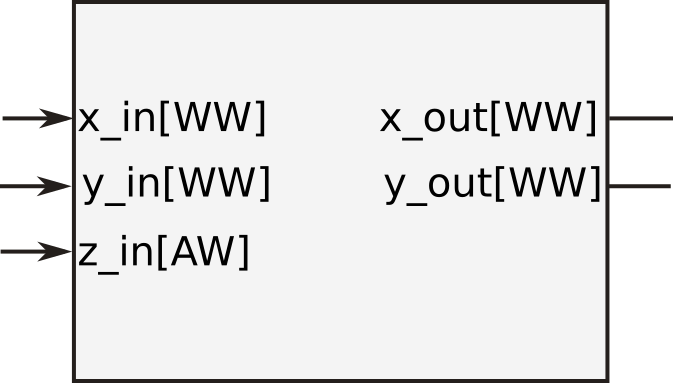
\includegraphics[width=7cm]{./figures/cordicDiam.png}
        \caption{Bloque de módulo de cómputo cordic}
        \label{fig:cordicDiam}
\end{figure}

Los parámetros \textit{WW} y \textit{AW} corresponden a los parámetros globales \textit{Word\_Width},
el ancho de palabra de las entradas de puntos, y \textit{Angle\_Width}, el ancho de palabra del
ángulo de rotación.

Al módulo cordic entra un punto complejo en forma de vector de dos componentes, y el ángulo de
rotación deseado, que representa el \textit{twiddle factor}. Es por esto que las unidades de control
de las dos arquitecturas radix implementadas generan los \textit{twiddle factors} en forma de
ángulos de rotación.
La salida del módulo cordic es el vector de dos dimensiones rotado en el ángulo indicado.\\

Como se indica en la subsección \ref{sec:cordicsec} el algoritmo cordic tiene una cierta ganancia
intrínseca que depende de la cantidad de iteraciones que se realizan. Como se desea que la ganancia
del algoritmo sea $1$ para no modificar la norma del vector de entrada se implementa un módulo de
escalamiento a la salida del módulo cordic para compensar la ganancia de la arquitectura. El valor
por el cual se escala la salida del módulo dependerá de la cantidad de iteraciones que se realicen,
que es un parámetro global de la arquitectura cordic.

Para facilitar la rotación de los vectores de entrada, primero se analiza el ángulo de rotación para
descomponerlo en un primer paso en rotaciones de $90^\circ$ y luego se utiliza el algoritmo cordic para
la rotación final menor al ángulo recto. De este modo, donde el algoritmo se aplica solo a
rotaciones menores a $90^\circ$, se obtienen resultados más precisos con menor cantidad de rotaciones.
También impacta en el tamaño total de la arquitectura, ya que se debe implementar una tabla con los
valores de los $\arctan(\alpha)$ para cada microrotación, por lo que a mayor número de iteraciones
posibles mayor tamaño de la tabla de arcotangentes.\\
Para esto se implementa un preprocesador que analiza el ángulo de entrada y genera las primeras
rotaciones de $90^\circ$, $180^\circ$ o $270^\circ$ sobre el vector de entrada, que consisten en intercambios de
las componentes y cambios de signos.

En la figura \ref{fig:cordicBlocks} se observa el diagrama en bloques interno del módulo de cómputo
cordic. El bloque \textit{Preprocessor} realiza el análisis del angúlo y las rotaciones iniciales de
$90^\circ$ en caso de ser necesarias. El bloque \textit{Unrolled cordic} realiza la rotación mediante el
algoritmo cordic, que se muestra detallado en la figura \ref{fig:uCordicBlocks}, y los bloques
\textit{Post mult.} realizan el escalamiento final para compensar la ganancia propia del algoritmo cordic.

\begin{figure}[htb!]
        \centering
        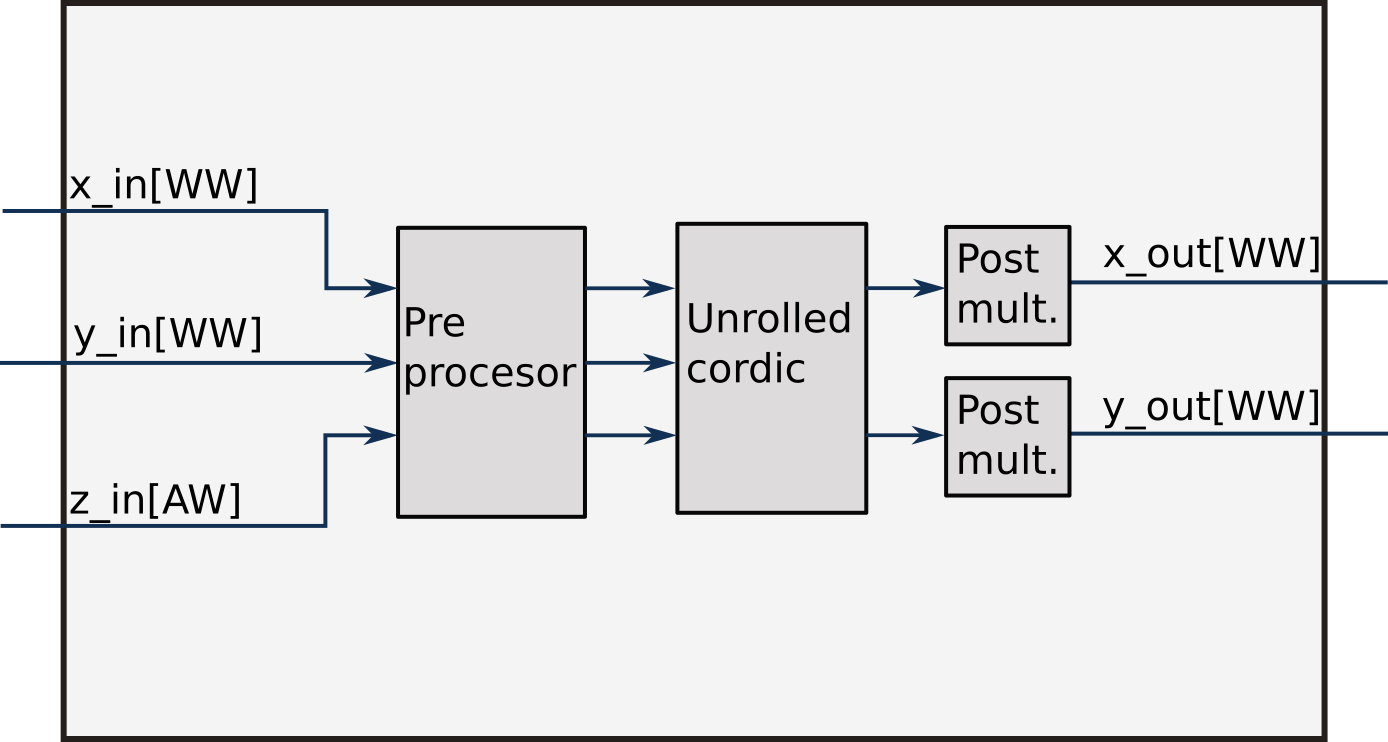
\includegraphics[width=9cm]{./figures/cordicBlocks.png}
        \caption{Diagrama en bloques del módulo cordic}
        \label{fig:cordicBlocks}
\end{figure}

\begin{figure}[htb!]
        \centering
        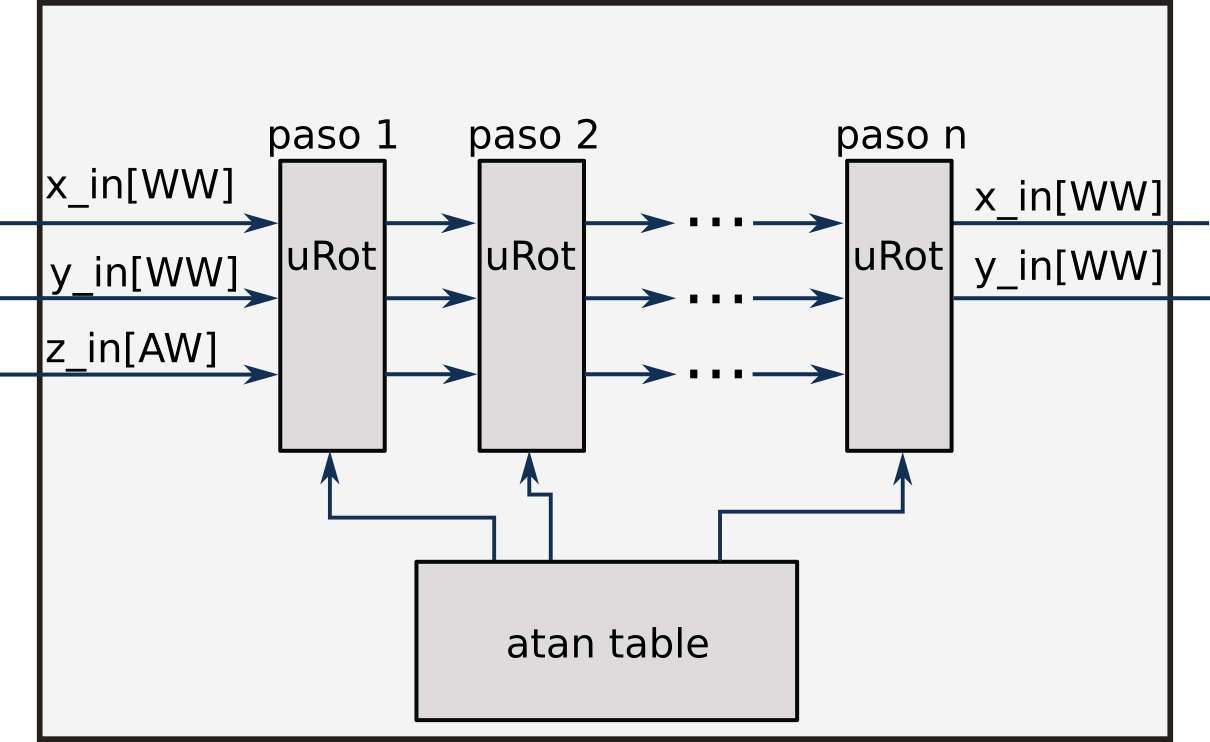
\includegraphics[width=9cm]{./figures/uCordicBlocks.png}
        \caption{Diagrama en bloques del bloque de rotaciones del módulo cordic}
        \label{fig:uCordicBlocks}
\end{figure}

Los bloques \textit{uRot} de la figura \ref{fig:uCordicBlocks} son los encargados de realizar las
microrotaciones sucesivas de acuerdo al algoritmo cordic. Los valores de los $\arctan(\alpha)$ se
almacenan previamente en la memoria \textit{atan table} de acuerdo a la cantidad de iteraciones que
se realizarán, y de allí son leídas por cada módulo de rotación.

\subsection{Multiplicador complejo}

La otra alternativa implementada para la multiplicación por los \textit{twiddle factors} es a través
de un multiplicador complejo. Para mantener la compatibilidad con el módulo cordic, y permitir que
la elección entre uno u otro sea transparente para el resto de las arquitecturas, se utilizan las
mismas interfaces en sus entradas y salidas, como se observa en la figura \ref{fig:multDiam}.

\begin{figure}[htb!]
        \centering
        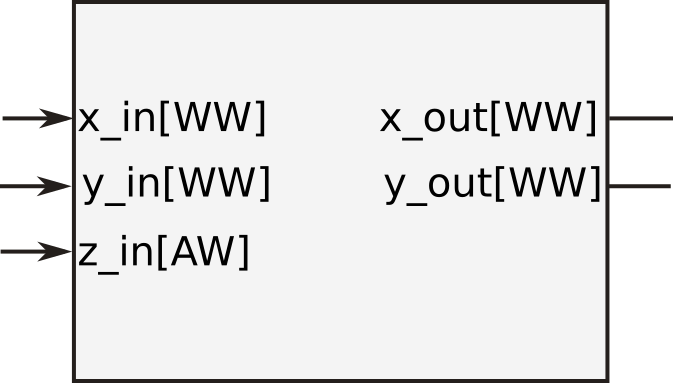
\includegraphics[width=7cm]{./figures/cordicDiam.png}
        \caption{Bloque de módulo multiplicador complejo}
        \label{fig:multDiam}
\end{figure}

El multiplicador recibe como entradas un vector de dos dimensiones, $x\_in$ e $y\_in$, y el ángulo
de rotación, $z\_in$, y entrega a las salidas el vector rotado en $x\_out$ e $y\_out$.

Para realizar la rotación a través de una multiplicación compleja, se almacenan los vectores
complejos correspondientes a cada ángulo posible de rotación en una memoria. Los vectores
almacenados tienen norma igual a $1$ de manera que no afecten la norma del vector de entrada.
Como los posibles ángulos de rotación son conocidos para una arquitectura y cantidad de puntos
dados, se ordenan en memoria de forma que esta sea direccionada por el valor del ángulo generado por
la unidad de control, obteniendo en cada posición el par de componentes del vector de norma $1$ que
corresponde al ángulo.\\
En la tabla \ref{table:angbits} se muestran ejemplos de la codificación binaria de
distintos ángulos para un ancho de palabra de ángulo de 7 bits.

\begin{table}[htb!]
\centering
\begin{tabular}{l c}
\textbf{Ángulo} & \textbf{Codificación binaria}\\ \hline 
$180^\circ$ & $100000$ \\
$90^\circ$ &  $0100000$ \\
$45^\circ$ &  $0010000$ \\
$135^\circ$ & $0110000$ \\ \hline
\end{tabular}
\caption{Ejemplos de codificación del ángulo para un ancho de palabra del ángulo de 7 bits}
\label{table:angbits}
\end{table}

Para reducir la cantidad de ángulos a almacenar se realiza un preprocesamiento previo donde se
analiza el ángulo y se realizan rotaciones iniciales en pasos de $90^\circ$ que consisten en intercambio
de las componentes y cambios de signo, que son operaciones triviales, y luego el ángulo restante
menor a $90^\circ$ se resuelve mediante la multiplicación compleja. De esta manera, en memoria solo deben
almacenarse ángulos menore a $90^\circ$.\\
Teniendo en cuenta que la variedad de ángulos a almacenar aumenta conforme aumenta la cantidad de
puntos para la que se instancia la arquitectura, y además esa variedad aumenta añadiendo ángulos de
tamaños cada vez menor, se implementa la tabla de forma que solo se crea del tamaño necesario para
la cantidad de puntos específica de la arquitectura particular que se está instanciando. Por ejemplo, para una arquitectura radix-2 de $16$ puntos, solo se necesita implementar la memoria con $4$
valores, incluyendo el ángulo $0$ en la posición de memoria $0$. En cambio para una radix-2 de $64$
puntos se necesitan $32$ valores de ángulos distintos almacenados en memoria.\\

Para direccionarlos se utiliza la palabra del ángulo trasladado al primer cuadrante invertida, de
modo que la posición de memoria correspondiente al ángulo $0$ es la $0$, la corresponfiente al
ángulo $45^\circ$ ($10\ldots0$) es la $1$ ($00\ldots01$), y así sucesivamente.\\

Al utilizar una transformación del ángulo a su vector normalizado correspondiente, no es necesario
un escalamiento luego de multiplicar.

\subsection{Unidad de escalamiento} \label{sec:secEscal}

La unidad de escalamiento de las unidades aritméticas de cada arquitectura permite realizar un
escalamiento del resultado de la operación aritmética en una o varias etapas seleccionadas en forma
dinámica, mediante una señal de entrada, para evitar posibles \textit{overflow} a lo largo del
cómputo de la FFT, ya que la aritmética de la arquitectura es de punto fijo en palabras de longitud
fija.\\

Las opciones de escalamiento disponibles, como se explicó en la subsección \ref{sec:redond}, son
redondeo y truncamiento.

En la figura \ref{fig:escBlocks} se muestra el diagrama en bloques de la unidad de escalamiento.

\begin{figure}[htb!]
        \centering
        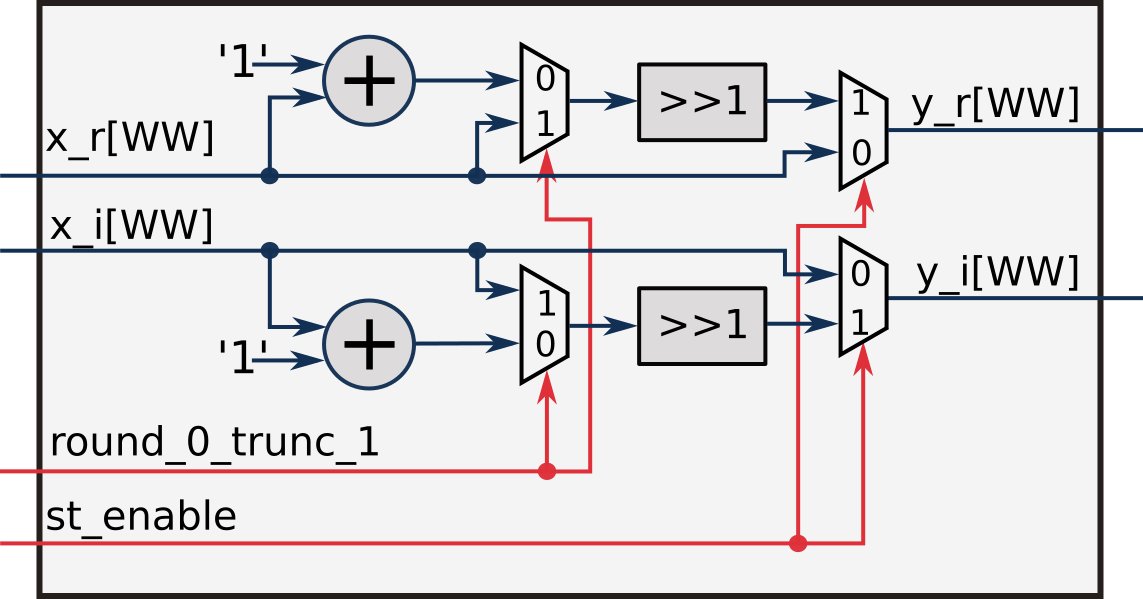
\includegraphics[width=9cm]{./figures/escBlocks.png}
        \caption{Diagrama en bloques de la unidad de escalamiento}
        \label{fig:escBlocks}
\end{figure}

La unidad le suma $1$ a cada una de las entradas. Con un multiplexor controlado por la señal
\textit{round\_0\_trunc\_1} se elige si se desplaza a derecha un bit la señal original o la salida
del sumador, eligiendo así entre truncamiento o redondeo respectivamente. Luego, la salida de la unidad
será la seña original, en caso de no estar habilitado el escalamiento para esa etapa, o la señal
desplazada, en caso de estar habilitado el escalamiento para esa etapa, realizando la selección
mediante dos multilpexores controlados por la señal \textit{st\_enable}.

\section{Interfaces de las arquitecturas}

Las dos arquitecturas implementadas tienen los mismos puertos de entrada y salida mostrados en la
figura \ref{fig:arqInterf}. 

\begin{figure}[htb!]
        \centering
        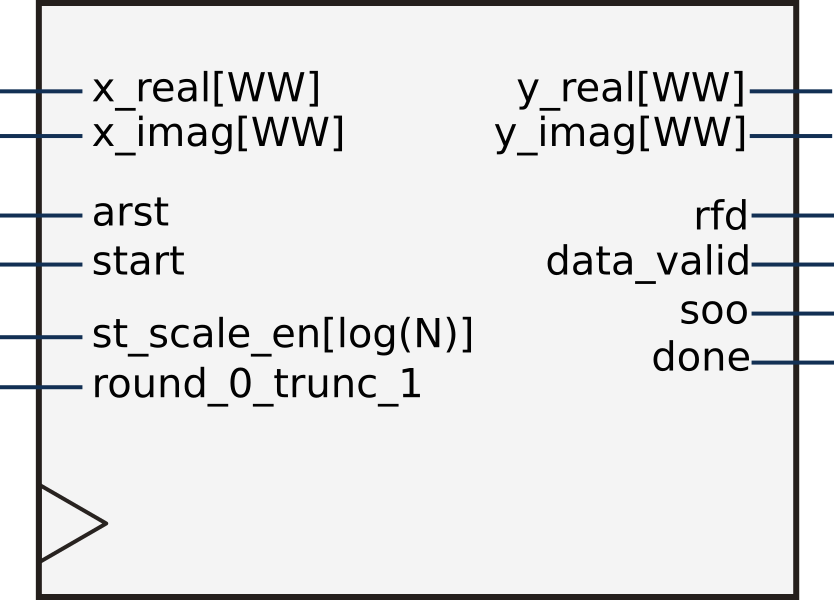
\includegraphics[width=8cm]{./figures/arcInterf.png}
        \caption{Señales de comunicación de las arquitecturas implementadas}
        \label{fig:arqInterf}
\end{figure}

Los puertos se describen en el siguiente listado:

\begin{itemize}
  \item \textbf{x\_real} ($WORD\_WIDTH$) componente real del punto de entrada.
  \item \textbf{x\_imag} ($WORD\_WIDTH$) componente imaginaria del punto de entrada.
  \item \textbf{arst} señal de reset asincrónico. Reinicia la arquitectura.
  \item \textbf{start} Señal de comienzo de funcionamiento luego de un reinicio. Al detectar la
  señal la arquitectura lee el primer dato de entrada y comienza con el cómputo de la primer FFT.
  \item \textbf{st\_scale\_en} ($(\log_\nu(N)))$) Habilitación del escalamiento posterior a la
  operación aritmética. Un $'1'$ en un bit habilita el escalamiento en la etapa correspondiente.
  \item \textbf{round\_0\_trunc\_1} Selección del tipo de escalamiento posterior a la operación
  aritmética, redondeo o truncamiento.
  \item \textbf{y\_real} ($WORD\_WIDTH$) componente real del punto de salida.
  \item \textbf{y\_imag} ($WORD\_WIDTH$) componente imaginaria del punto de salida.
  \item \textbf{rfd} señal que indica que debe colocarse un nuevo punto en la entrada de la
  arquitectura.
  \item \textbf{data\_valid} señal que indica que el dato presente en la salida es válido.
  \item \textbf{soo} señal que indica que el dato presente en la salida es el primero de una nueva
  FFT.
  \item \textbf{done} señal que indica que el dato presente en la salida es el último de la actual
  FFT.
\end{itemize}

Se listan a continuación los parámetros globales de las arquitecturas implementadas.

\begin{itemize}
  \item \textbf{WORD\_WIDTH} Cantidad de bits de codificación de los puntos de entrada y salida.
  \item \textbf{CLOG2\_FFT\_POINTS} Logaritmo, en base dos, de la cantidad de puntos para la que es
  implementada la arquitectura. A través de este parámetro se infiere dentro de la arquitectura la
  cantidad de puntos de la FFT a procesar.
  \item \textbf{FFT\_1\_IFFT\_0} selección de implementación de la arquitectura para realizar FFT o
  IFFT.
  \item \textbf{ANGLE\_WIDTH} Cantidad de bits de codificación de los ángulos de representación de
  los \textit{twiddle factors}.
\end{itemize}

\section{Herramientas utilizadas para el desarrollo} \label{sec:herrSec}
% En el capítulo anterior se analizaron diferentes tipos de arquitecturas existentes para la implementación de un procesador de descomposición QR. Se describieron sus características a nivel conceptual y se detallaron las definiciones de la implementación elegida para realizar la implementación.
% 
% En este capítulo se describen las herramientas que fueron utilizadas y se explica en detalle, a nivel de microarquitectura, la forma en la cual fue implementado cada módulo del procesador desarrollado, y la forma en la cual los módulos son interconectados para conformar al mismo. Adicionalmente, se describen aquellas definiciones y desarrollos que fueron el resultado de la presente tesis, utilizados para resolver diferentes necesidades encontradas, los cuales representan un contenido intelectual propio.
% 
% La metodología utilizada para el desarrollo del procesador consistió en analizar las necesidades de la arquitectura elegida, y los diferentes componentes requeridos. Se procedió a la definición de dicha arquitectura a través de un diagrama en bloques y se desarrolló cada uno de los módulos por separado, gradualmente. Una vez desarrollado un módulo, se procedíó a simular su comportamiento aislado a través de un testbench que lograra contemplar la mayor parte de los posibles vectores de entrada. Una vez finalizada la simulación individual de los distintos componentes, se procedó a realizar una simulación conjunta de algunos de ellos.
% 
% \section{Herramientas utilizadas}
% 
 A continuación se hace una breve reseña de las herramientas utilizadas para la implementación de
 las arquitecturas:
 
\subsubsection*{Sublime Text 2}
\begin{wrapfigure}{r}{0.22\textwidth}
	\vspace{-15pt}
	\begin{center}
		
\includegraphics[width=0.20\textwidth]{./figures/logo_sublime.png}
	\end{center}
	\vspace{-15pt}
\end{wrapfigure}
Sublime fue el editor de texto utilizado para codificar en lenguaje Verilog. El mismo presenta una
interfaz gráfica con diferentes características de gran utilidad, marcado de palabras claves,
autocompletado, etc.

% \subsubsection*{Vim}
% \begin{wrapfigure}{r}{0.22\textwidth}
% 	\vspace{-20pt}
% 	\begin{center}
% 		\includegraphics[width=0.15\textwidth]{./figures/logo_vim.png}
% 	\end{center}
% 	\vspace{-20pt}
% \end{wrapfigure}
% Vim es un editor de texto nativo de entornos de tipo UNIX y fue utilizado en algunos casos en conjunto con Sublime Text 2.
% 
\subsubsection*{ModelSim}
\begin{wrapfigure}{r}{0.22\textwidth}
	\vspace{-15pt}
	\begin{center}
		
\includegraphics[width=0.20\textwidth]{./figures/logo_modelsim.png}
	\end{center}
	\vspace{-15pt}
\end{wrapfigure}
ModelSim fue la herramienta utilizada para la simulación de los códigos descriptos en Verilog, con
los cuales se generaron archivos de tipo wave de salida.

\subsubsection*{gtkwave}
\begin{wrapfigure}{r}{0.22\textwidth}
	\vspace{-15pt}
	\begin{center}
		
\includegraphics[width=0.20\textwidth]{./figures/logo_gtkwave.png}
	\end{center}
	\vspace{-15pt}
\end{wrapfigure}
Gtkwave fue la herramienta utilizada para visualizar los archivos de tipo wave que fueron generados
durante las simulaciones realizadas en ModelSim.

\subsubsection*{Xilinx ISE}
\begin{wrapfigure}{r}{0.22\textwidth}
	\vspace{-15pt}
	\begin{center}
		
\includegraphics[width=0.15\textwidth]{./figures/logo_ise.png}
	\end{center}
	\vspace{-15pt}
\end{wrapfigure}
Xilinx ISE es la herramienta proporcionada por la compañía Xilinx para crear los archivos de
síntesis ``.bit'' a partir de un hardware codificado en un lenguaje HDL, para ser implementado en
los dispositivos FPGA que provee. También fue utilizada para transferir los archivos ``.bit'' al
kit de desarrollo FPGA.

\subsubsection*{Bitbucket/Mercurial}
\begin{wrapfigure}{r}{0.22\textwidth}
	\vspace{-15pt}
	\begin{center}
		
\includegraphics[width=0.20\textwidth]{./figures/logo_bitbucket.png}
	\end{center}
	\vspace{-15pt}
\end{wrapfigure}
Para realizar el desarrollo se utilizó un repositorio hospedado en
\href{http://www.bitbucket.org}{http://www.bitbucket.org}, el cual fue utilizado a través de la
herramienta de versionado Mercurial. Dicho sistema aportó diversas ventajas, entre las cuales
principalmente se encuentran el mantener un registro de todas las modificaciones realizadas entre
cada una de las versiones y el poder trabajar en la nube.
